\documentclass{Configuration_Files/PoliMi3i_thesis}

%------------------------------------------------------------------------------
%	REQUIRED PACKAGES AND  CONFIGURATIONS
%------------------------------------------------------------------------------

% CONFIGURATIONS
\usepackage{parskip} % For paragraph layout
\usepackage{setspace} % For using single or double spacing
\usepackage{emptypage} % To insert empty pages
\usepackage{multicol} % To write in multiple columns (executive summary)
\setlength\columnsep{15pt} % Column separation in executive summary
\setlength\parindent{0pt} % Indentation
\raggedbottom  

% PACKAGES FOR TITLES
\usepackage{titlesec}
% \titlespacing{\section}{left spacing}{before spacing}{after spacing}
\titlespacing{\section}{0pt}{3.3ex}{2ex}
\titlespacing{\subsection}{0pt}{3.3ex}{1.65ex}
\titlespacing{\subsubsection}{0pt}{3.3ex}{1ex}
\usepackage{color}

% PACKAGES FOR LANGUAGE AND FONT
\usepackage[english]{babel} % The document is in English  
\usepackage[utf8]{inputenc} % UTF8 encoding
\usepackage[T1]{fontenc} % Font encoding
\usepackage[11pt]{moresize} % Big fonts

% PACKAGES FOR IMAGES
\usepackage{graphicx}
\usepackage{transparent} % Enables transparent images
\usepackage{eso-pic} % For the background picture on the title page
\usepackage{subfig} % Numbered and caption subfigures using \subfloat.
\usepackage{tikz} % A package for high-quality hand-made figures.
\usetikzlibrary{}
\graphicspath{{./Images/}} % Directory of the images
\usepackage{caption} % Coloured captions
\usepackage{xcolor} % Coloured captions
\usepackage{amsthm,thmtools,xcolor} % Coloured "Theorem"
\usepackage{float}

% STANDARD MATH PACKAGES
\usepackage{amsmath}
\usepackage{amsthm}
\usepackage{amssymb}
\usepackage{amsfonts}
\usepackage{bm}
\usepackage[overload]{empheq} % For braced-style systems of equations.
\usepackage{fix-cm} % To override original LaTeX restrictions on sizes

% PACKAGES FOR TABLES
\usepackage{tabularx}
\usepackage{longtable} % Tables that can span several pages
\usepackage{colortbl}

% PACKAGES FOR ALGORITHMS (PSEUDO-CODE)
\usepackage{algorithm}
\usepackage{algorithmic}

% PACKAGES FOR REFERENCES & BIBLIOGRAPHY
\usepackage[colorlinks=true,linkcolor=black,anchorcolor=black,citecolor=black,filecolor=black,menucolor=black,runcolor=black,urlcolor=black]{hyperref} % Adds clickable links at references
\usepackage{cleveref}
\usepackage[square, numbers, sort&compress]{natbib} % Square brackets, citing references with numbers, citations sorted by appearance in the text and compressed
\bibliographystyle{abbrvnat} % You may use a different style adapted to your field

% OTHER PACKAGES
\usepackage{pdfpages} % To include a pdf file
\usepackage{afterpage}
\usepackage{lipsum} % DUMMY PACKAGE
\usepackage{fancyhdr} % For the headers
\fancyhf{}

% Input of configuration file. Do not change config.tex file unless you really know what you are doing. 
% Define blue color typical of polimi
\definecolor{bluepoli}{cmyk}{0.4,0.1,0,0.4}

% Custom theorem environments
\declaretheoremstyle[
  headfont=\color{bluepoli}\normalfont\bfseries,
  bodyfont=\color{black}\normalfont\itshape,
]{colored}

% Set-up caption colors
\captionsetup[figure]{labelfont={color=bluepoli}} % Set colour of the captions
\captionsetup[table]{labelfont={color=bluepoli}} % Set colour of the captions
\captionsetup[algorithm]{labelfont={color=bluepoli}} % Set colour of the captions

\theoremstyle{colored}
\newtheorem{theorem}{Theorem}[chapter]
\newtheorem{proposition}{Proposition}[chapter]

% Enhances the features of the standard "table" and "tabular" environments.
\newcommand\T{\rule{0pt}{2.6ex}}
\newcommand\B{\rule[-1.2ex]{0pt}{0pt}}

% Pseudo-code algorithm descriptions.
\newcounter{algsubstate}
\renewcommand{\thealgsubstate}{\alph{algsubstate}}
\newenvironment{algsubstates}
  {\setcounter{algsubstate}{0}%
   \renewcommand{\STATE}{%
     \stepcounter{algsubstate}%
     \Statex {\small\thealgsubstate:}\space}}
  {}

% New font size
\newcommand\numfontsize{\@setfontsize\Huge{200}{60}}

% Title format: chapter
\titleformat{\chapter}[hang]{
\fontsize{50}{20}\selectfont\bfseries\filright}{\textcolor{bluepoli} \thechapter\hsp\hspace{2mm}\textcolor{bluepoli}{|   }\hsp}{0pt}{\huge\bfseries \textcolor{bluepoli}
}

% Title format: section
\titleformat{\section}
{\color{bluepoli}\normalfont\Large\bfseries}
{\color{bluepoli}\thesection.}{1em}{}

% Title format: subsection
\titleformat{\subsection}
{\color{bluepoli}\normalfont\large\bfseries}
{\color{bluepoli}\thesubsection.}{1em}{}

% Title format: subsubsection
\titleformat{\subsubsection}
{\color{bluepoli}\normalfont\large\bfseries}
{\color{bluepoli}\thesubsubsection.}{1em}{}

% Shortening for setting no horizontal-spacing
\newcommand{\hsp}{\hspace{0pt}}

\makeatletter
% Renewcommand: cleardoublepage including the background pic
\renewcommand*\cleardoublepage{%
  \clearpage\if@twoside\ifodd\c@page\else
  \null
  \AddToShipoutPicture*{\BackgroundPic}
  \thispagestyle{empty}%
  \newpage
  \if@twocolumn\hbox{}\newpage\fi\fi\fi}
\makeatother

%For correctly numbering algorithms
\numberwithin{algorithm}{chapter}

%----------------------------------------------------------------------------
%	NEW COMMANDS DEFINED
%----------------------------------------------------------------------------

% EXAMPLES OF NEW COMMANDS
\newcommand{\bea}{\begin{eqnarray}} % Shortcut for equation arrays
\newcommand{\eea}{\end{eqnarray}}
\newcommand{\e}[1]{\times 10^{#1}}  % Powers of 10 notation

%----------------------------------------------------------------------------
%	ADD YOUR PACKAGES (be careful of package interaction)
%----------------------------------------------------------------------------

%----------------------------------------------------------------------------
%	ADD YOUR DEFINITIONS AND COMMANDS (be careful of existing commands)
%----------------------------------------------------------------------------

%----------------------------------------------------------------------------
%	BEGIN OF YOUR DOCUMENT
%----------------------------------------------------------------------------

\begin{document}

\fancypagestyle{plain}{%
\fancyhf{} % Clear all header and footer fields
\fancyhead[RO,RE]{\thepage} %RO=right odd, RE=right even
\renewcommand{\headrulewidth}{0pt}
\renewcommand{\footrulewidth}{0pt}}

%----------------------------------------------------------------------------
%	TITLE PAGE
%----------------------------------------------------------------------------

\pagestyle{empty} % No page numbers
\frontmatter % Use roman page numbering style (i, ii, iii, iv...) for the preamble pages

\puttitle{
	title=Systems and Methods for Big and Unstructured Data Project,
	name1=Edoardo Silvio Gribaldo (11086870), % Author Name and Surname
    name2=, 
	name3=, 
	name4=,
	name5=,
	academicyear=2024-2025,
	groupnumber=30
} % These info will be put into your Title page 

%----------------------------------------------------------------------------
%	PREAMBLE PAGES: ABSTRACT (inglese e italiano), EXECUTIVE SUMMARY
%----------------------------------------------------------------------------
\startpreamble
\setcounter{page}{1} % Set page counter to 1

%----------------------------------------------------------------------------
%	LIST OF CONTENTS/FIGURES/TABLES/SYMBOLS
%----------------------------------------------------------------------------

% TABLE OF CONTENTS
\thispagestyle{empty}
\tableofcontents % Table of contents 
\thispagestyle{empty}
\cleardoublepage

%-------------------------------------------------------------------------
%	THESIS MAIN TEXT
%-------------------------------------------------------------------------
% In the main text of your thesis you can write the chapters in two different ways:
%
% (1) As presented in this template you can write:
%    \chapter{Title of the chapter}
%    *body of the chapter*

% (2) You can write your chapter in a separated .tex file and then include it in the main file with the following command:
%    \chapter{Title of the chapter}
%    \input{chapter_file.tex}
%
% Especially for long thesis, we recommend you the second option.

\addtocontents{toc}{\vspace{2em}} % Add a gap in the Contents, for aesthetics
\mainmatter % Begin numeric (1,2,3...) page numbering

\chapter{Introduction}
The goal of this document is to analyze and extract useful information from the dataset available at:
\newline 
\href{https://www.kaggle.com/datasets/juhibhojani/airline-reviews}{https://www.kaggle.com/datasets/juhibhojani/airline-reviews}
\section{Problems to address}
I would like to extrapolate information from this dataset in order to suggest data driven decision to airlines that could enhance their customer experience. To do so I will try to search any correlation between the satisfaction (or dissatisfaction) of people that wrote the reviews. 

\section {Why Elasticsearch?}

First of all, being the info mostly present in natural language in the text of the reviews, I will have to resort to indexing and ranking of textual reviews. That is the main reason behind the choice of Elasticsearch. Indeed it is a really flexible technology capable not only of handling huge dataset but also of indexing and ranking documents (in this case the reviews) to perform text analysis with the queries. Moreover, I will also exploit the ability of Elasticsearch to perform queries with date ranges to see some correlation between time and the a certain sentiment of the reviews.
%\label{ch:chapter_one}%
% The \label{...}% enables to remove the small indentation that is generated, always leave the % symbol.

%In this chapter additional useful information are reported.

\chapter{Data Wrangling}
I had to clean a little bit the dataset. To do that I imported the zipped file on Colab and performed a simple exploration on the data as well.
The Colab notebook is available at the following link:
\newline
\href{https://github.com/edogriba/SMBUD-2024/blob/main/DataWrangling.ipynb}{https://github.com/edogriba/SMBUD-2024/blob/main/DataWrangling.ipynb}
\newline
I performed the following steps: 
\begin{enumerate}
    \item I got a glimpse of the dataset using df.head()
    \item I checked the types of the columns
    \item I checked which columns had null values.
    \item I thought If could fill some of those values but I believed that would have changed too much the dataset and I didn't do it
    \item Since I had troubles with boolean types while uploading the .csv file on Elasticsearch I had to change the value from boolean True/False to text 'true'/'false' in order to make them recognizable as boolean values by Elasticsearch.
    \item I changed the 'Review Date' field into date type
    \item I printed the output to a a new .csv file
\end{enumerate}
The following is the Python script I wrote for doing that:
\begin{verbatim}
!unzip Airline_review.csv.zip

import numpy as np
import pandas as pd

df = pd.read_csv('Airline_review.csv')
df.head()

print(df.isnull().sum())

print(df.dtypes == 'bool')

df.loc[df["Verified"] == True, "Verified"] = "true"
df.loc[df["Verified"] == False, "Verified"] = "false"

df["Review Date"] = pd.to_datetime(df["Review Date"], format="%dth %B %Y", errors="coerce")

df.to_csv("output.csv", index=False)
\end{verbatim}


\chapter{Dataset}
The choice of the dataset was not really easy. Since I am using Elasticsearch I was looking for a dataset who had some text to be analyzed. I ended up choosing the airlines review dataset for many reasons. First of all, it is a medium size dataset. Indeed the free version of  Elasticsearch allowed me only to upload files of maximum 500 MB and many interesting databases were GBs of data. Moreover the .csv format made it simpler to explore and clean a little bit the data with a simple script in Python. Another thing to underline is that there were a lot of datasets with reviews that had only 2 columns (the review and the sentiment), clearly used to train models to predict the sentiment of a review. Of course no such dataset would have been useful for my purpose. Indeed I needed about a dozen of different columns to be able to perform 10 valuable queries. 
Now, regarding the dataset, it is composed by reviews of flights made by several airlines. This is the manual mapping that I did
\begin{verbatim}
{
  "properties": {
    "Aircraft": {
      "type": "keyword"
    },
    "Airline Name": {
      "type": "keyword"
    },
    "Cabin Staff Service": {
      "type": "integer"
    },
    "Date Flown": {
      "type": "keyword"
    },
    "Food & Beverages": {
      "type": "integer"
    },
    "Ground Service": {
      "type": "integer"
    },
    "Inflight Entertainment": {
      "type": "integer"
    },
    "Overall_Rating": {
      "type": "integer"
    },
    "Recommended": {
      "type": "boolean"
    },
    "Review": {
      "type": "text"
    },
    "Review Date": {
      "type": "date",
      "format": "iso8601"
    },
    "Review_Title": {
      "type": "text"
    },
    "Route": {
      "type": "text"
    },
    "Seat Comfort": {
      "type": "integer"
    },
    "Seat Type": {
      "type": "keyword"
    },
    "Type Of Traveller": {
      "type": "keyword"
    },
    "Id": {
      "type": "long"
    },
    "Value For Money": {
      "type": "double"
    },
    "Verified": {
      "type": "boolean"
    },
    "Wifi \& Connectivity": {
      "type": "double"
    }
  }
}
\end{verbatim}
The reason behind this type of mapping is straightforward. 
\begin{enumerate}
    \item The Id column is mapped as a long
    \item All the columns that contain numbers are mapped to integer
    \item All the columns that contain variables that can be assigned values of a closed domain are mapped as keywords. 
    The Flown Date in the original dataset was in the format [textual month][integer year] so it was impossible to recover the precise flown date and I preferred storing it as text. Of course the Review Date is not before the Flown Date but I cannot be sure if it is the actual date of the flight or some days later so I preferred to map it as a keyword (to make a query grouping by the month and the year) and keep it separate from the Review Date that will be used to make range queries.
    \item All the columns containing textual content are mapped to text. 
    \item The Review Date column is mapped as a date for obvious reasons
    \item The Recommended and Verified columns are boolean for obvious reasons
    
\end{enumerate}


\chapter{Queries}

\begin{enumerate}
%1
    \item Get the average overall rating for different types of travellers who reviewed their trip in the year 2022

\begin{verbatim}
GET airlines/_search
{
  "size": 0,
  "query": {
    "bool": {
      "must": [
        {
          "range": {
            "Review Date": {
              "gte": "2022-01-01",
              "lte": "2022-12-31"
            }
          }
        }
      ],
      "must_not": [
        {
          "term": {
            "Type Of Traveller": "Unknown"
          }
        }
      ]
    }
  },
  "aggs": {
    "avg_rating_by_class": {
      "terms": {
        "field": "Type Of Traveller"
      },
      "aggs": {
        "avg_rating": {
          "avg": {
            "field": "Overall_Rating"
          }
        }
      }
    }
  }
}

\end{verbatim}

\newpage

\begin{figure}[H]
    \centering
    \subfloat{
        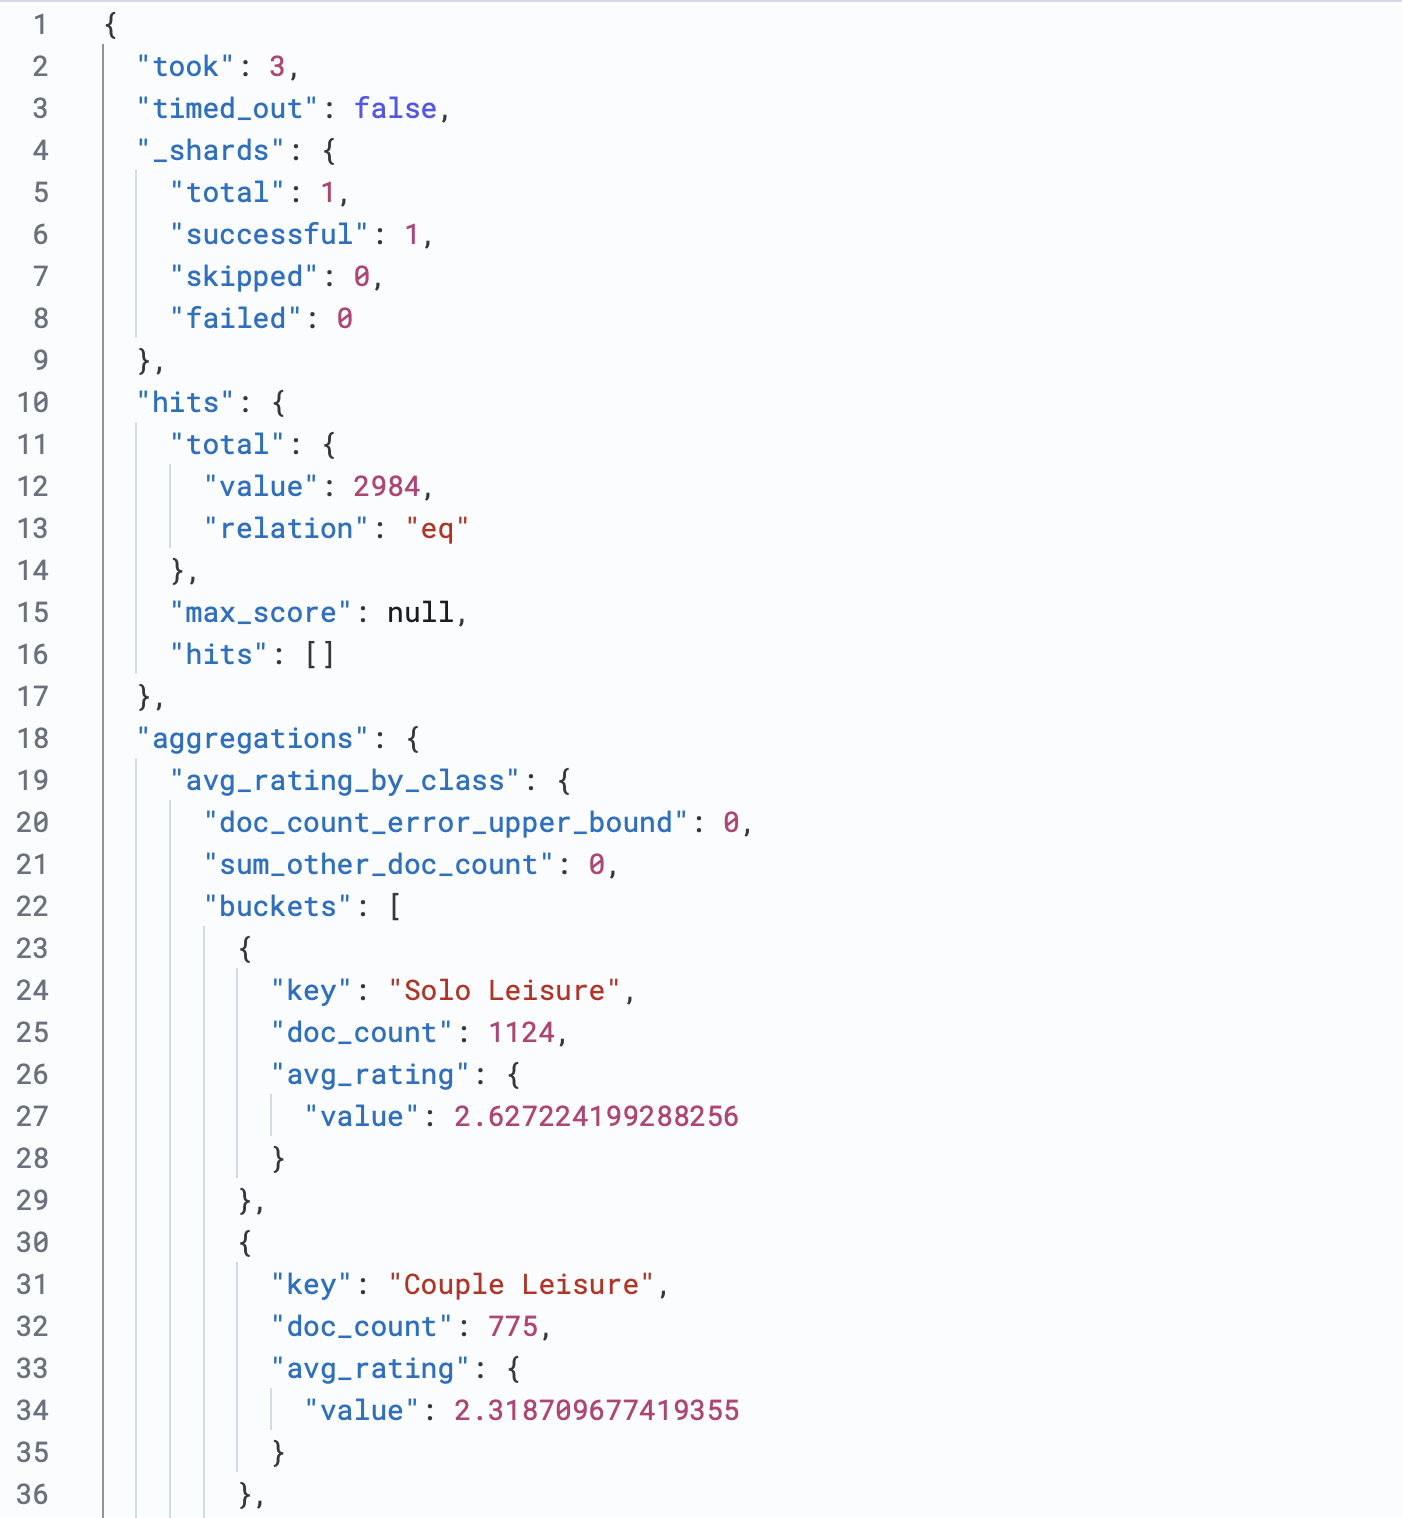
\includegraphics[scale=0.5]{Images/QueryResults/query1a.png}
    }
    \quad
    \subfloat{
        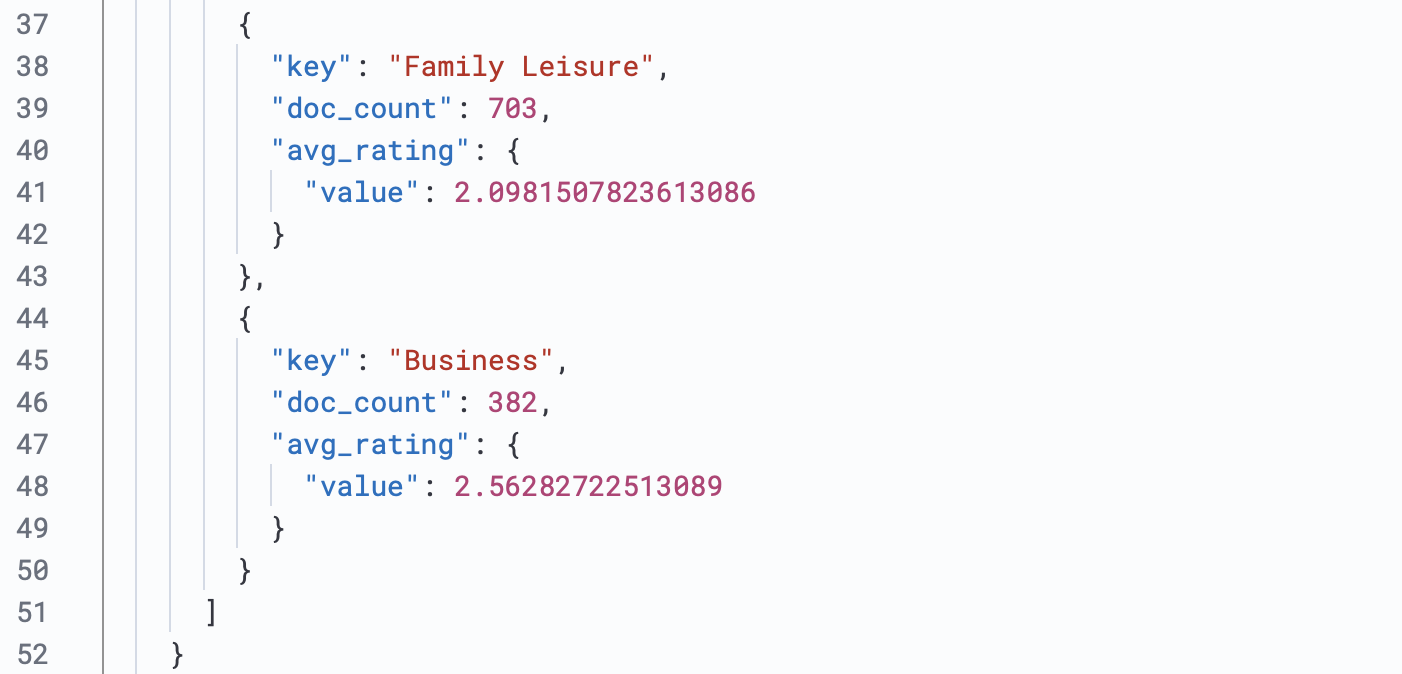
\includegraphics[scale=0.5]{Images/QueryResults/query1b.png}
    }
    \label{fig:quadtree2}
    \caption{Results from Query 1}

\end{figure}
\newpage

    \item Get the list of reviews about business class trips that included a tasty meal with a rating of 4 or more on the category Food \& Beverages (boost it by 4). It's a plus if the review also said mentioned the comfort.


\begin{verbatim}
GET airlines/_search
{
  "size": 5, 
  "query": {
    "bool": {
      "filter": {
        "term": {
          "Seat Type": "Business Class"
        }
      },
      "must": [
        {
          "match": {
            "Review": {
              "query": "Tasty Meal",
              "boost": 4.0
            }
          }
        },
        {
          "range": {
            "Food & Beverages": {
              "gte": 4
            }
          }
        }
      ],
      "should": {
        "match": {
          "Review": "Comfort"
        }
      }, 
      "must_not": {
        "match": {
          "Review": "Decent"
        }
      }
    }
  }
}
\end{verbatim}

\newpage
\begin{figure}[H]
    \centering
    \subfloat{
        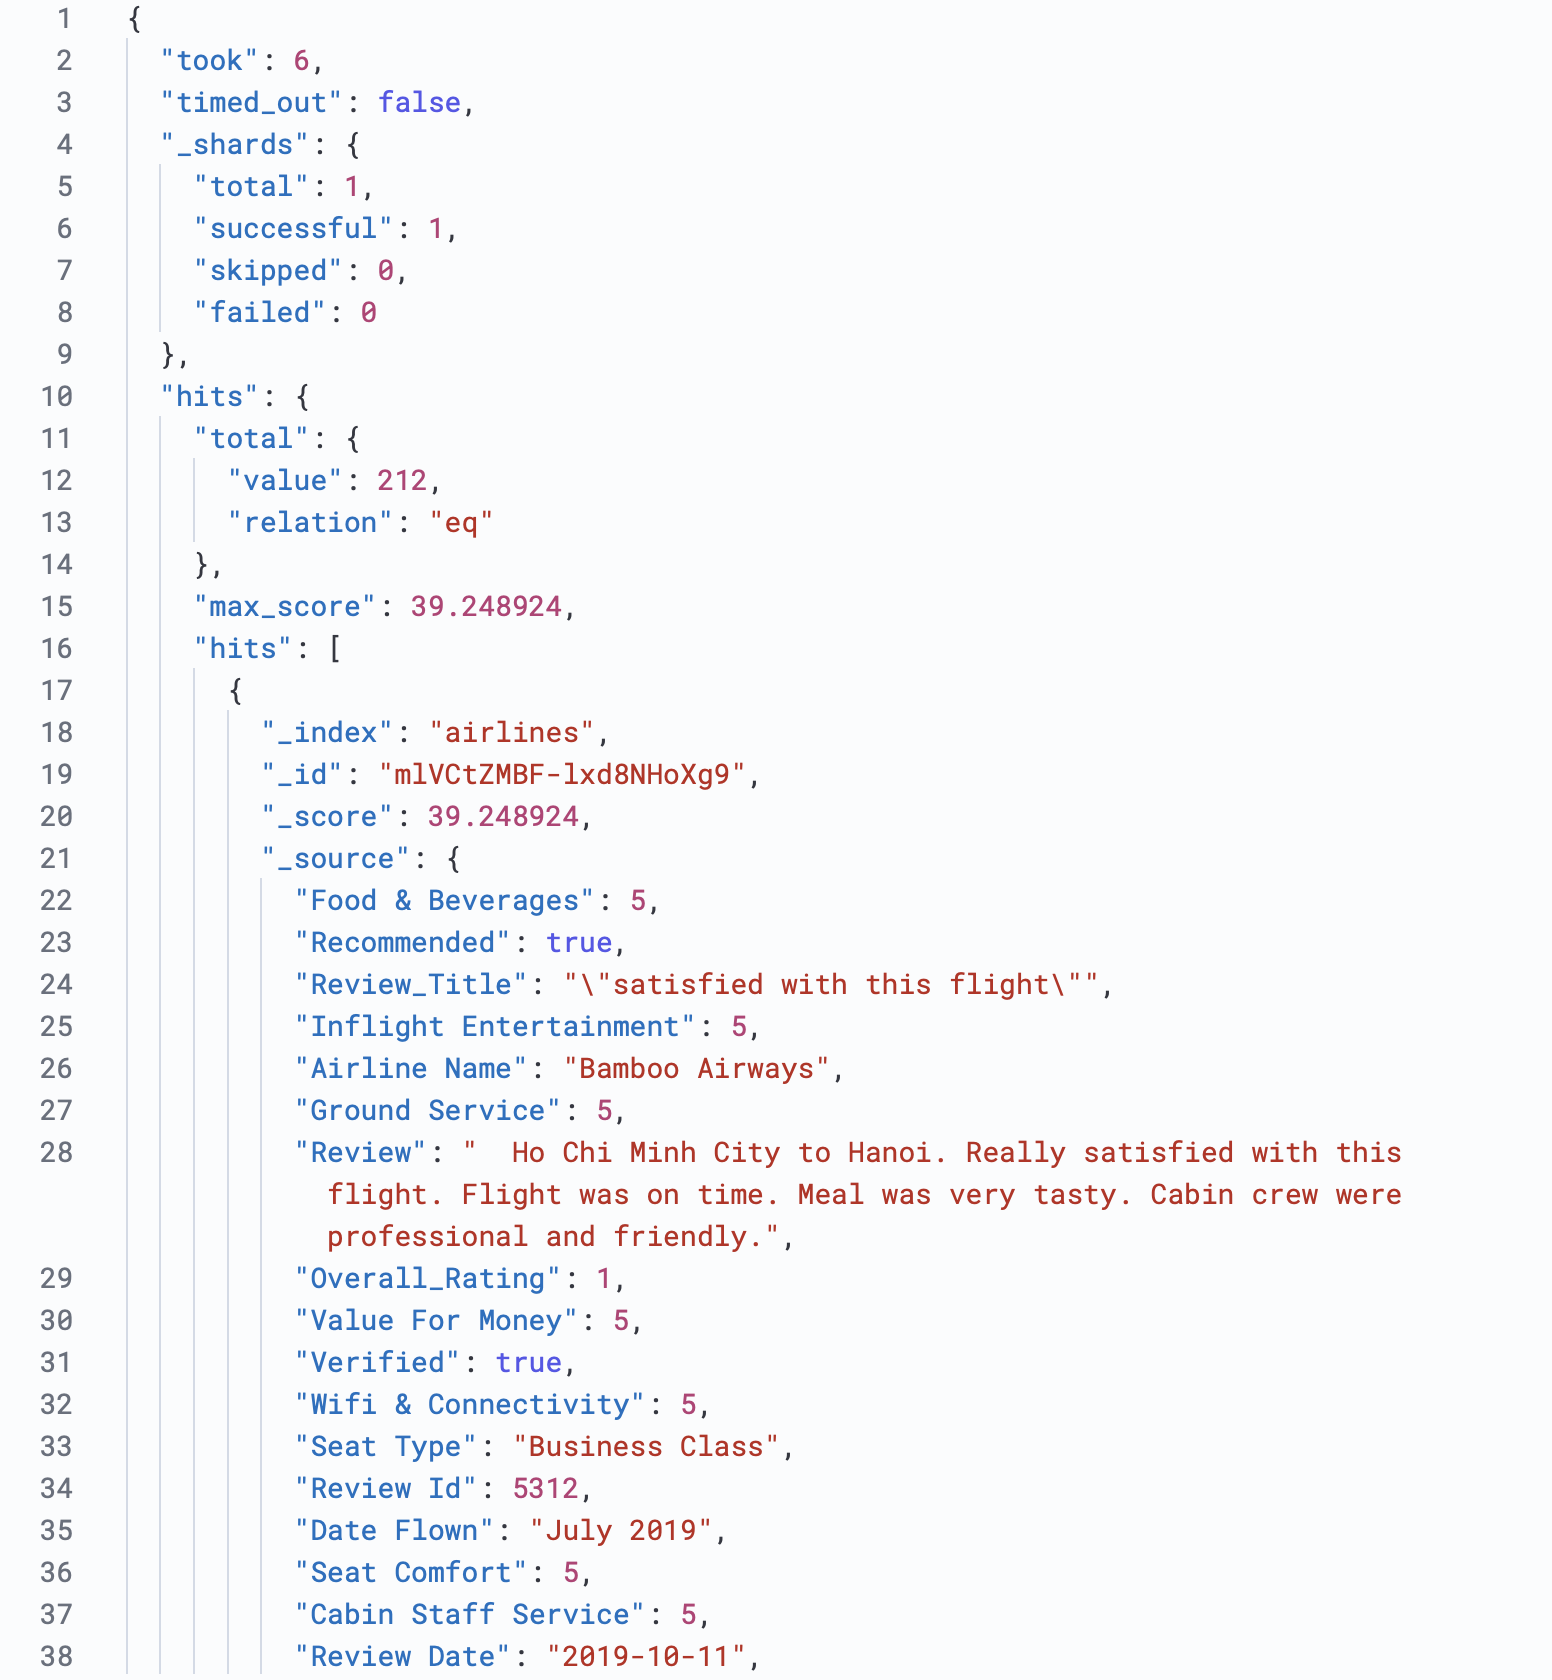
\includegraphics[scale=0.30]{Images/QueryResults/query2a.png}
    }
    \subfloat{
        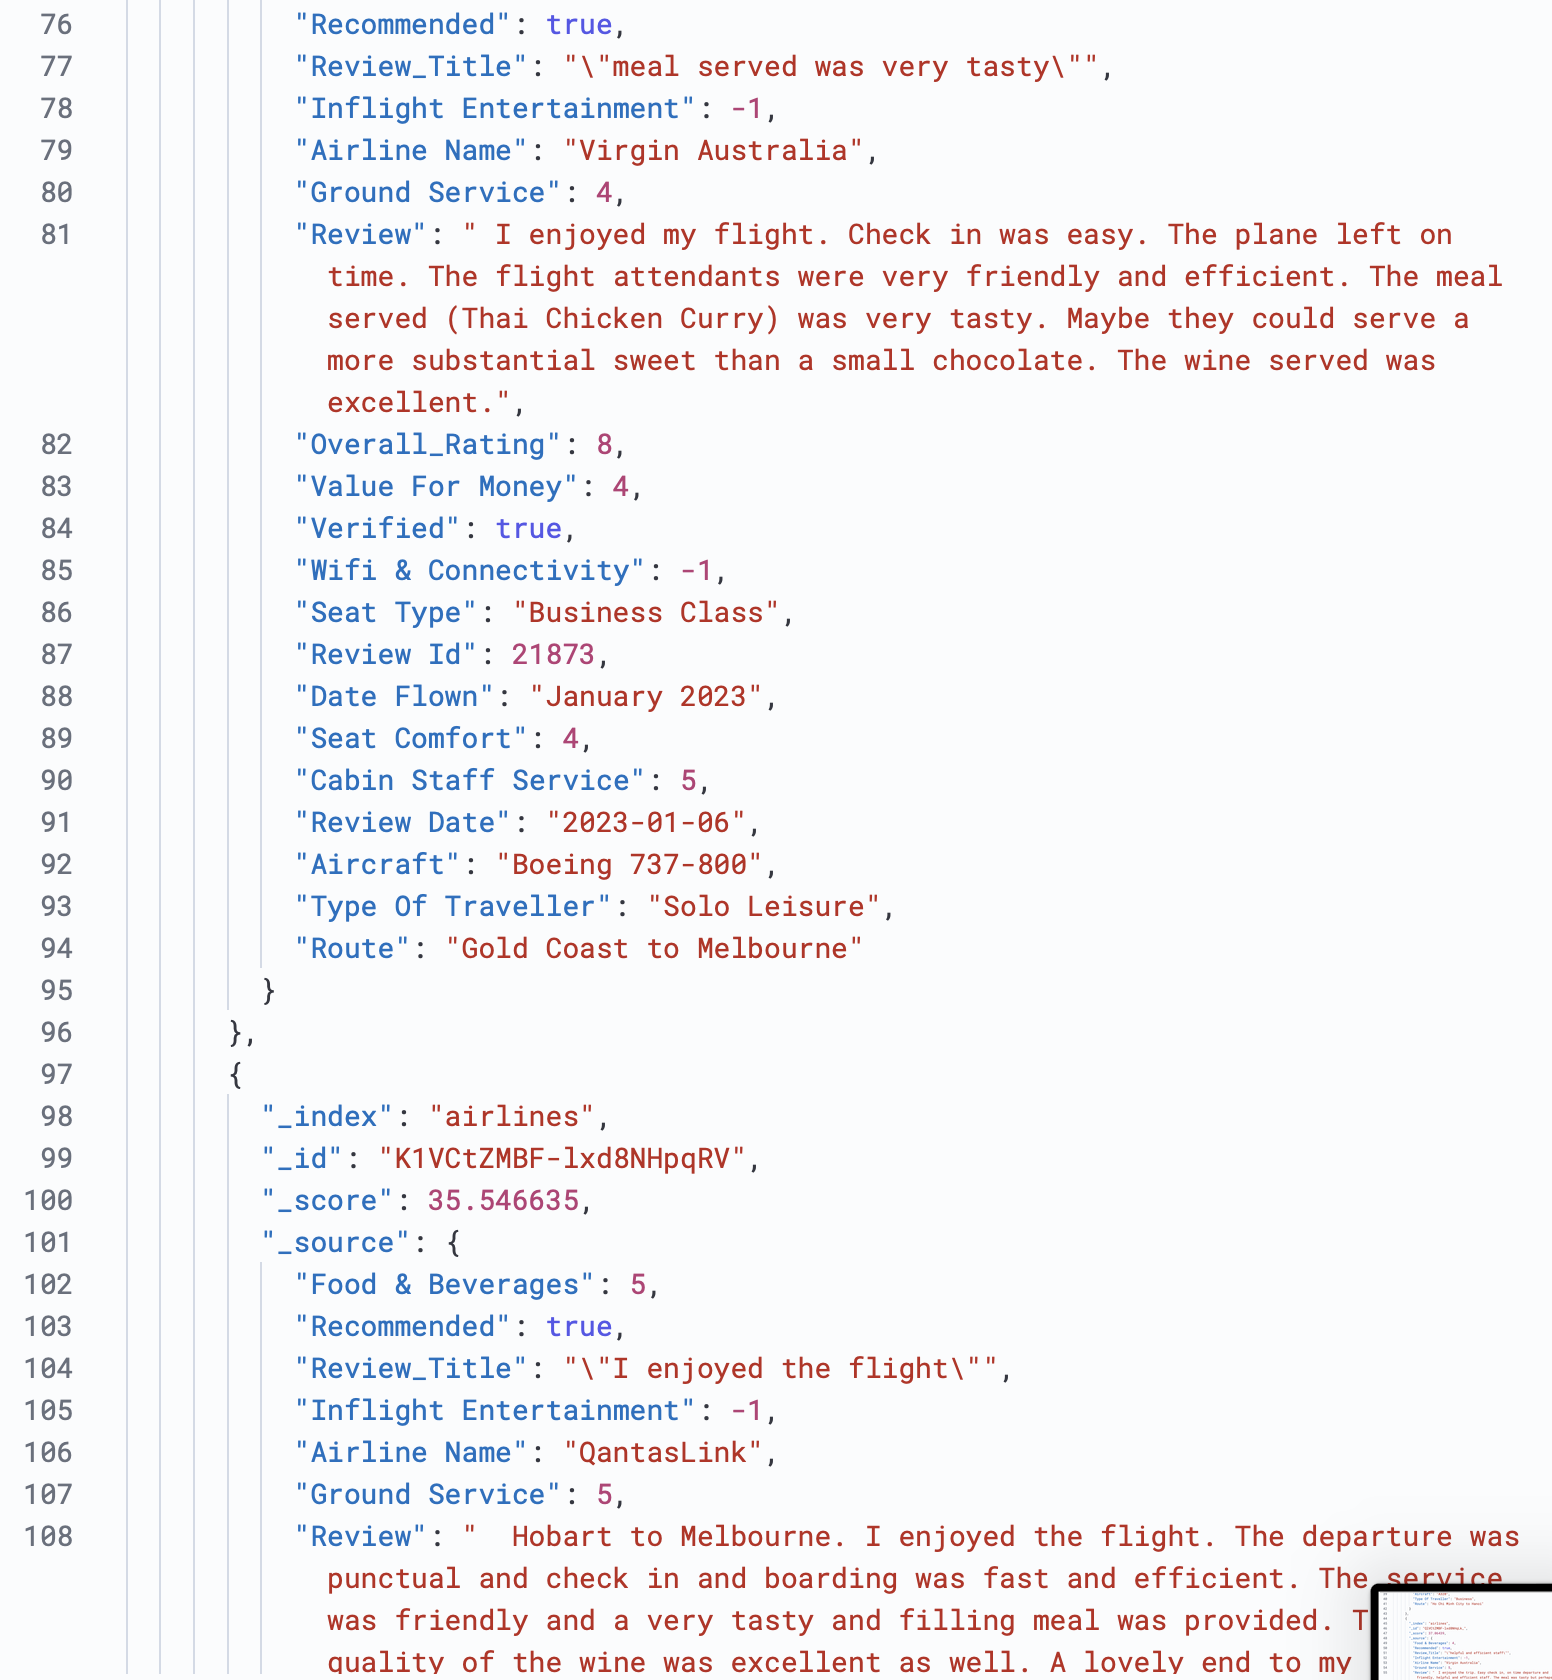
\includegraphics[scale=0.30]{Images/QueryResults/query2c.png}
    }
    \quad
    \subfloat{
        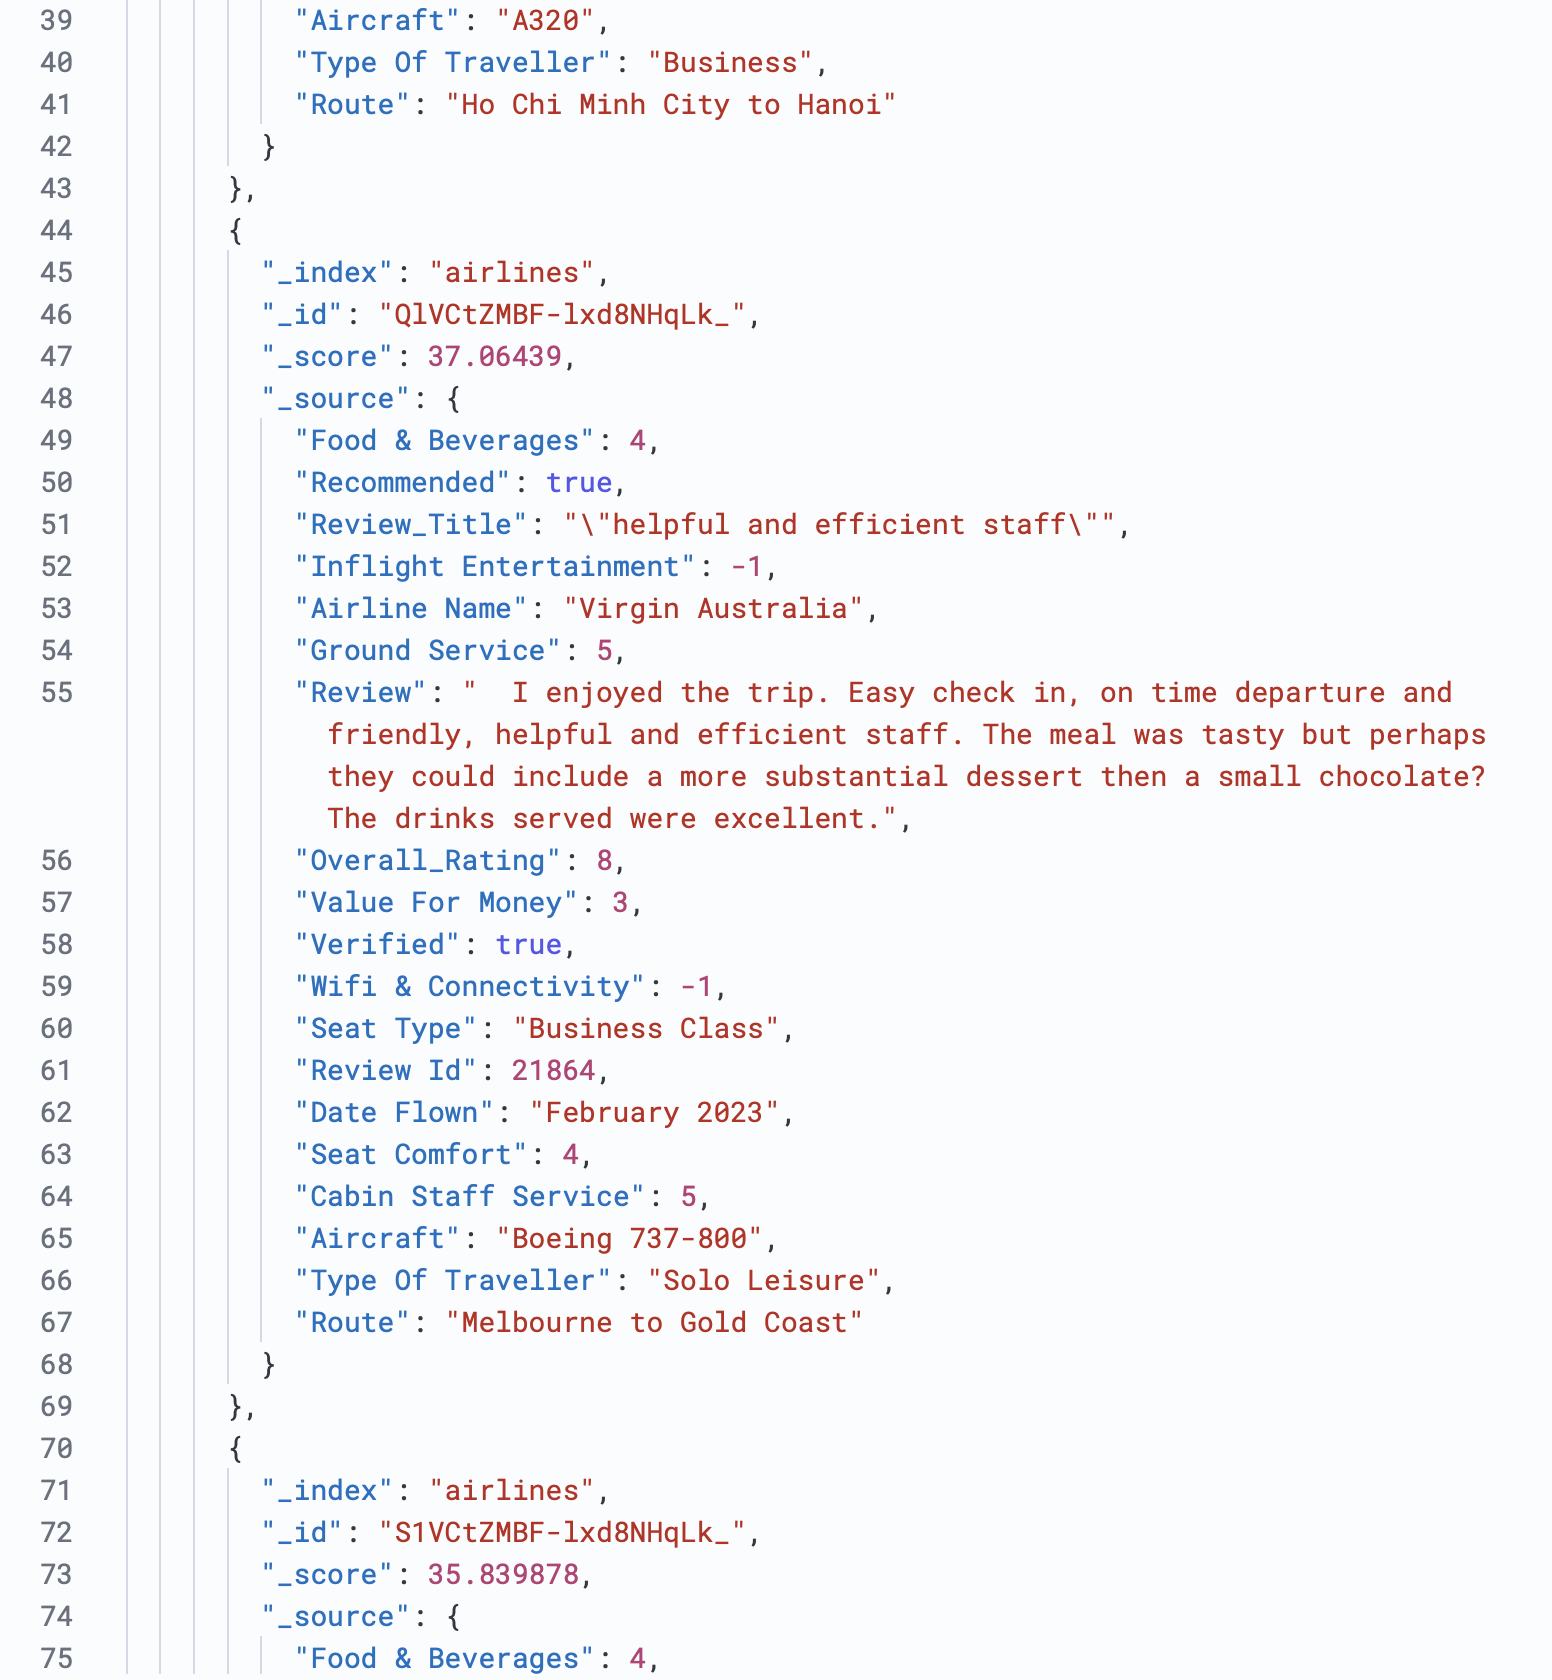
\includegraphics[scale=0.30]{Images/QueryResults/query2b.png}
    }
    \subfloat{
        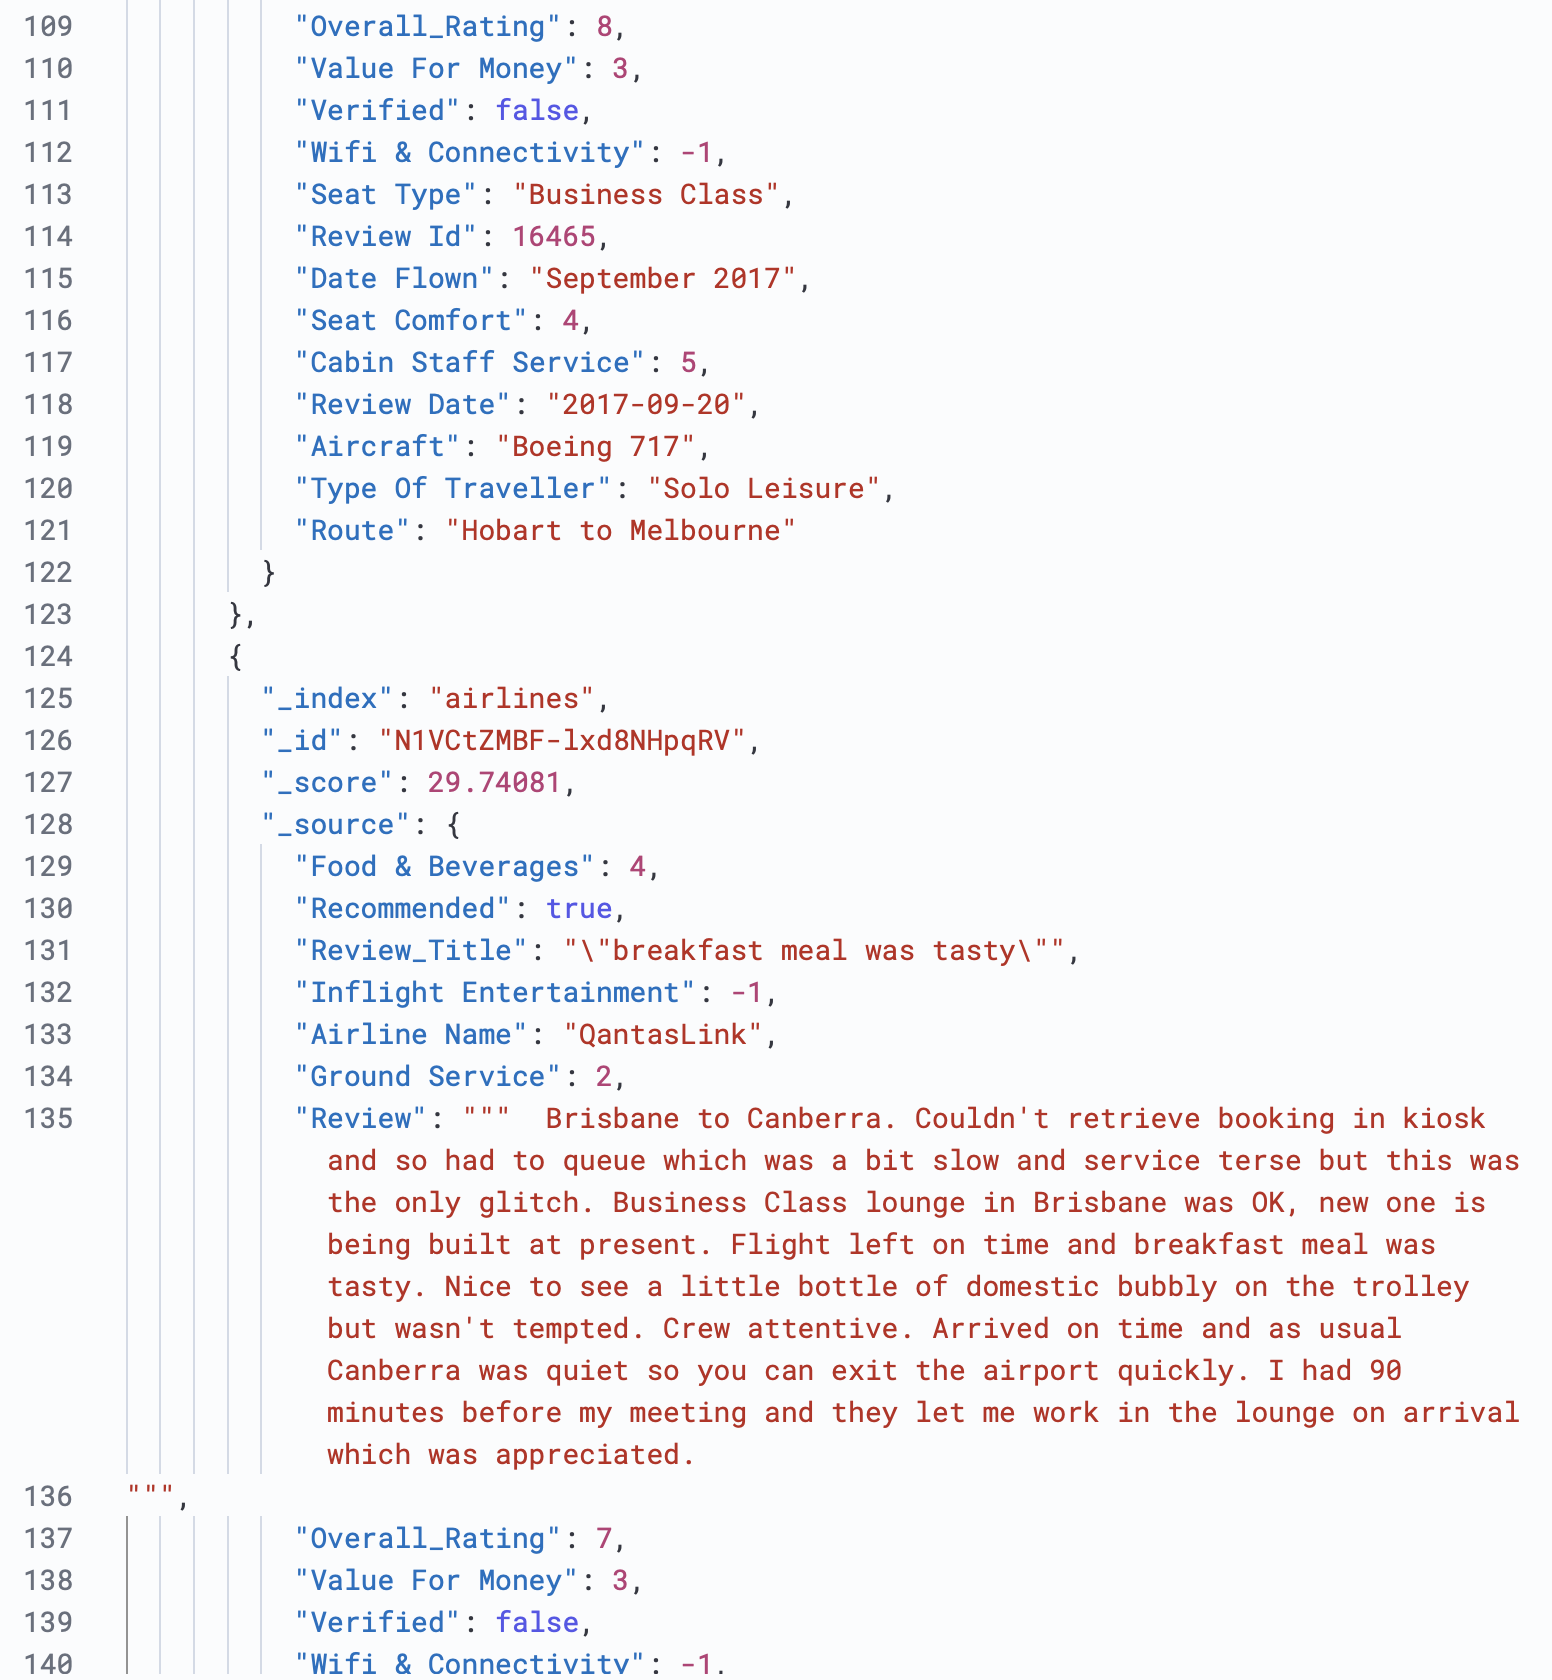
\includegraphics[scale=0.30]{Images/QueryResults/query2d.png}
    }
    \hfill    
    \subfloat{
        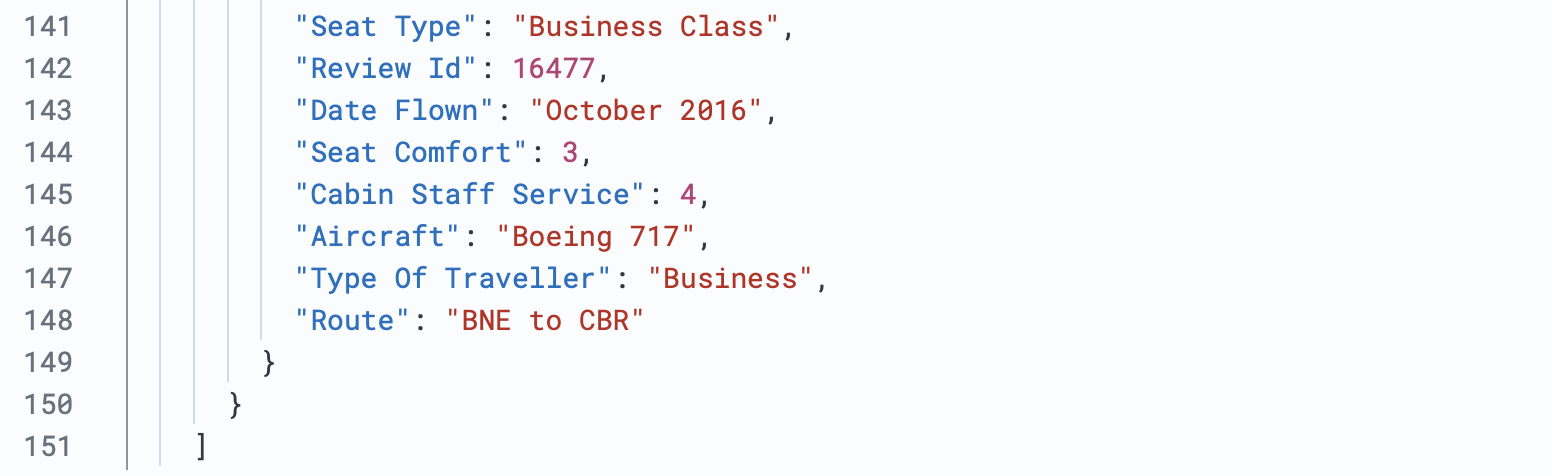
\includegraphics[scale=0.30]{Images/QueryResults/query2e.png}
    }
    \label{fig:quadtree2}
    \caption{Results from Query 2}

\end{figure}

\newpage

    \item Get the list of the airlines names and their respective number of reviews that recommend an airline written after 12/02/2020 and the 12/12/23, talking about Covid and having Cabin Staff Service and Ground Service both rated 3 or more
\begin{verbatim}
GET airlines/_search
{
  "size": 0,
  "query": {
    "bool": {
    "must": [
      {
        "range": {
          "Review Date":{
            "gte":  "2020-02-14",
            "lte": "2023-12-12"
          }
        }
      },
      {
        "match": {
          "Review": "Covid"
        }
      },
      {
        "match": {
          "Recommended": true
        }
      },
      {
        "range": {
          "Cabin Staff Service": {
            "gte": 3
          }
        }
      }, 
      {
        "range": {
          "Ground Service": {
            "gte": 3
          }
        }
      }
    ]
    }
  },
  "aggs": {
    "lost_per_airlines": {
      "terms": {
        "field": "Airline Name"
      }
    }
  }
}
\end{verbatim}
    

\begin{figure}[H]
    \centering
    \subfloat{
        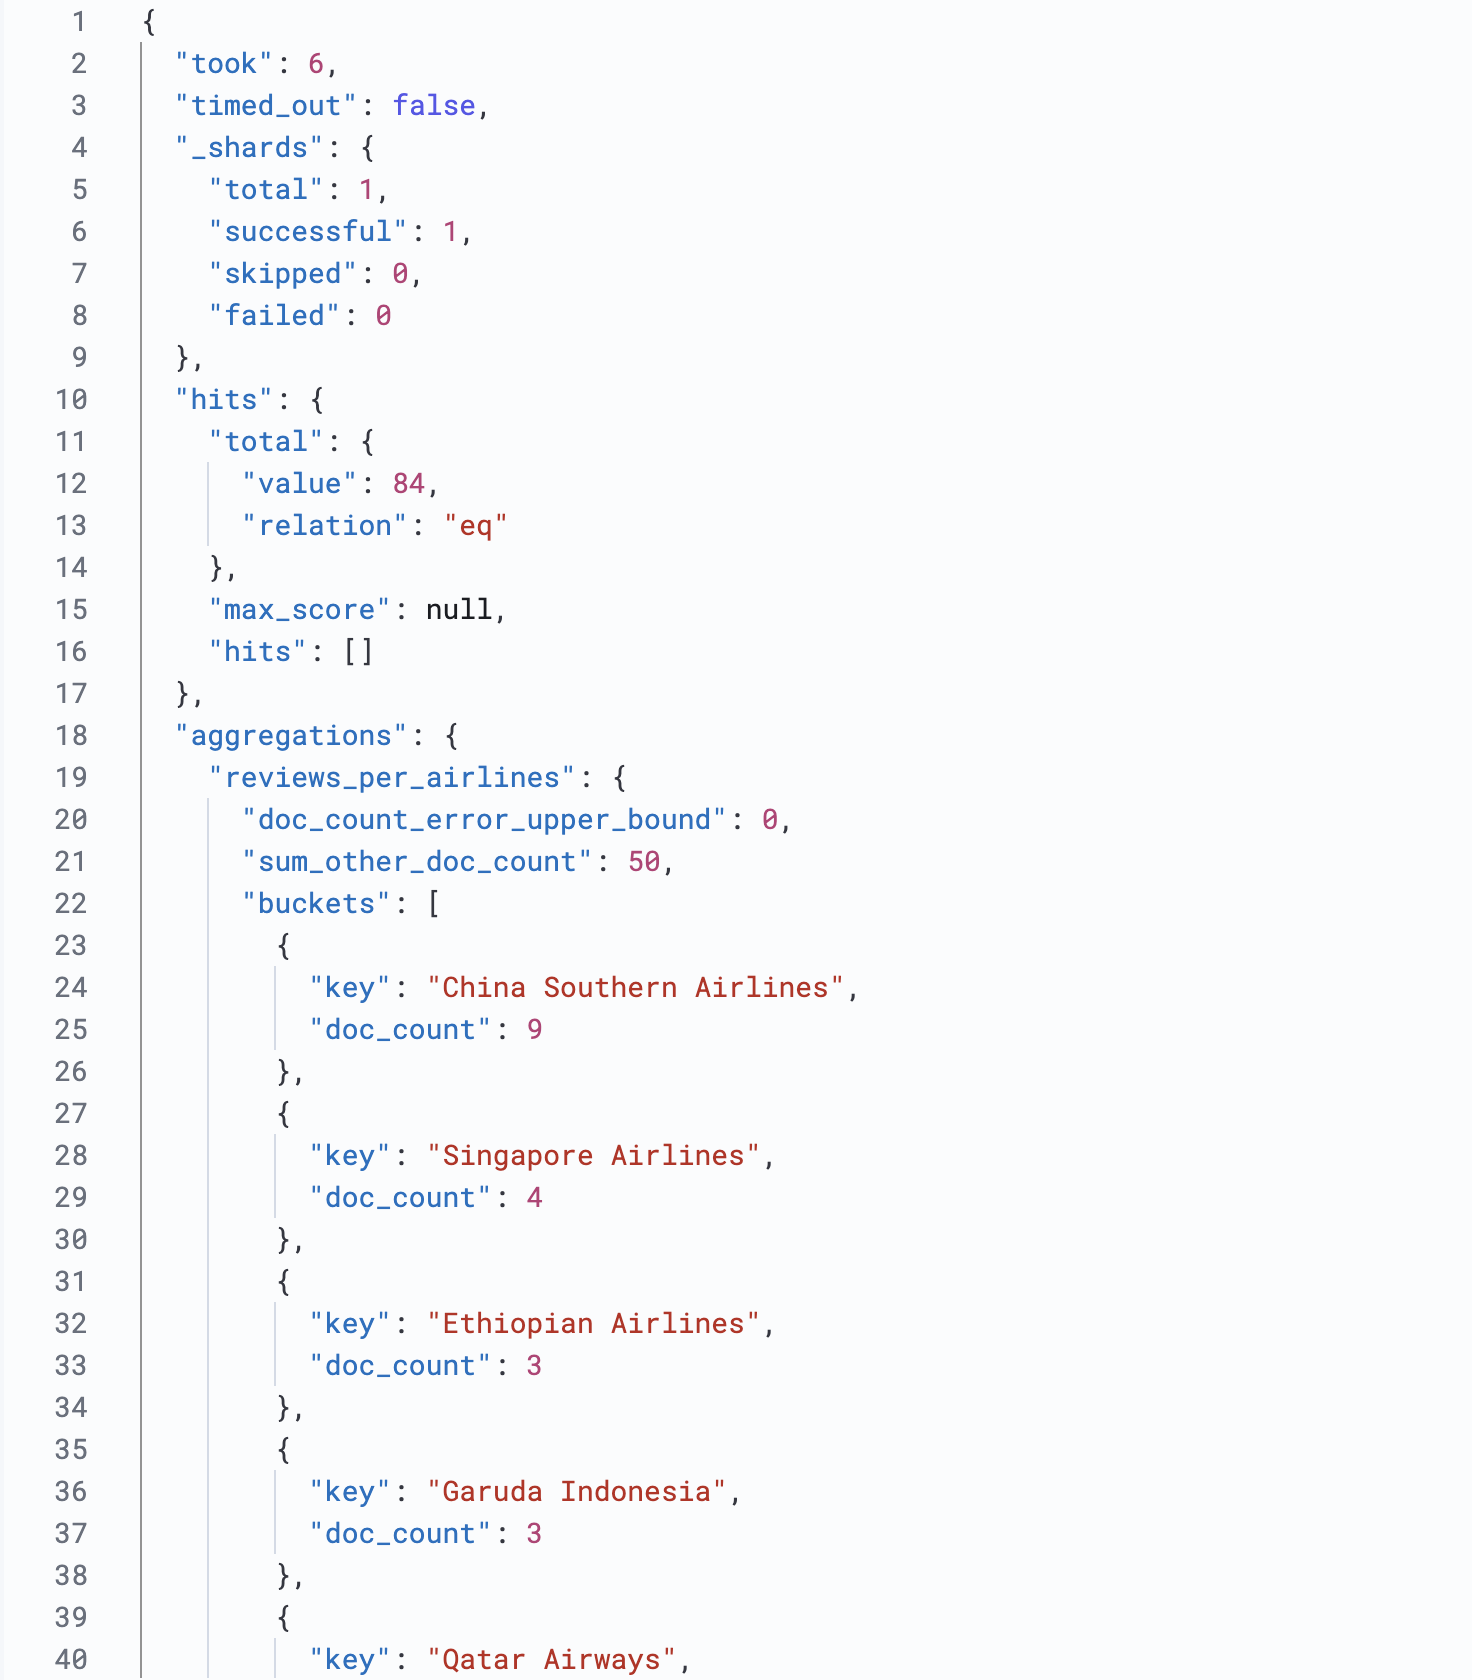
\includegraphics[scale=0.50]{Images/QueryResults/query3a.png}
    }\\
    \subfloat{
        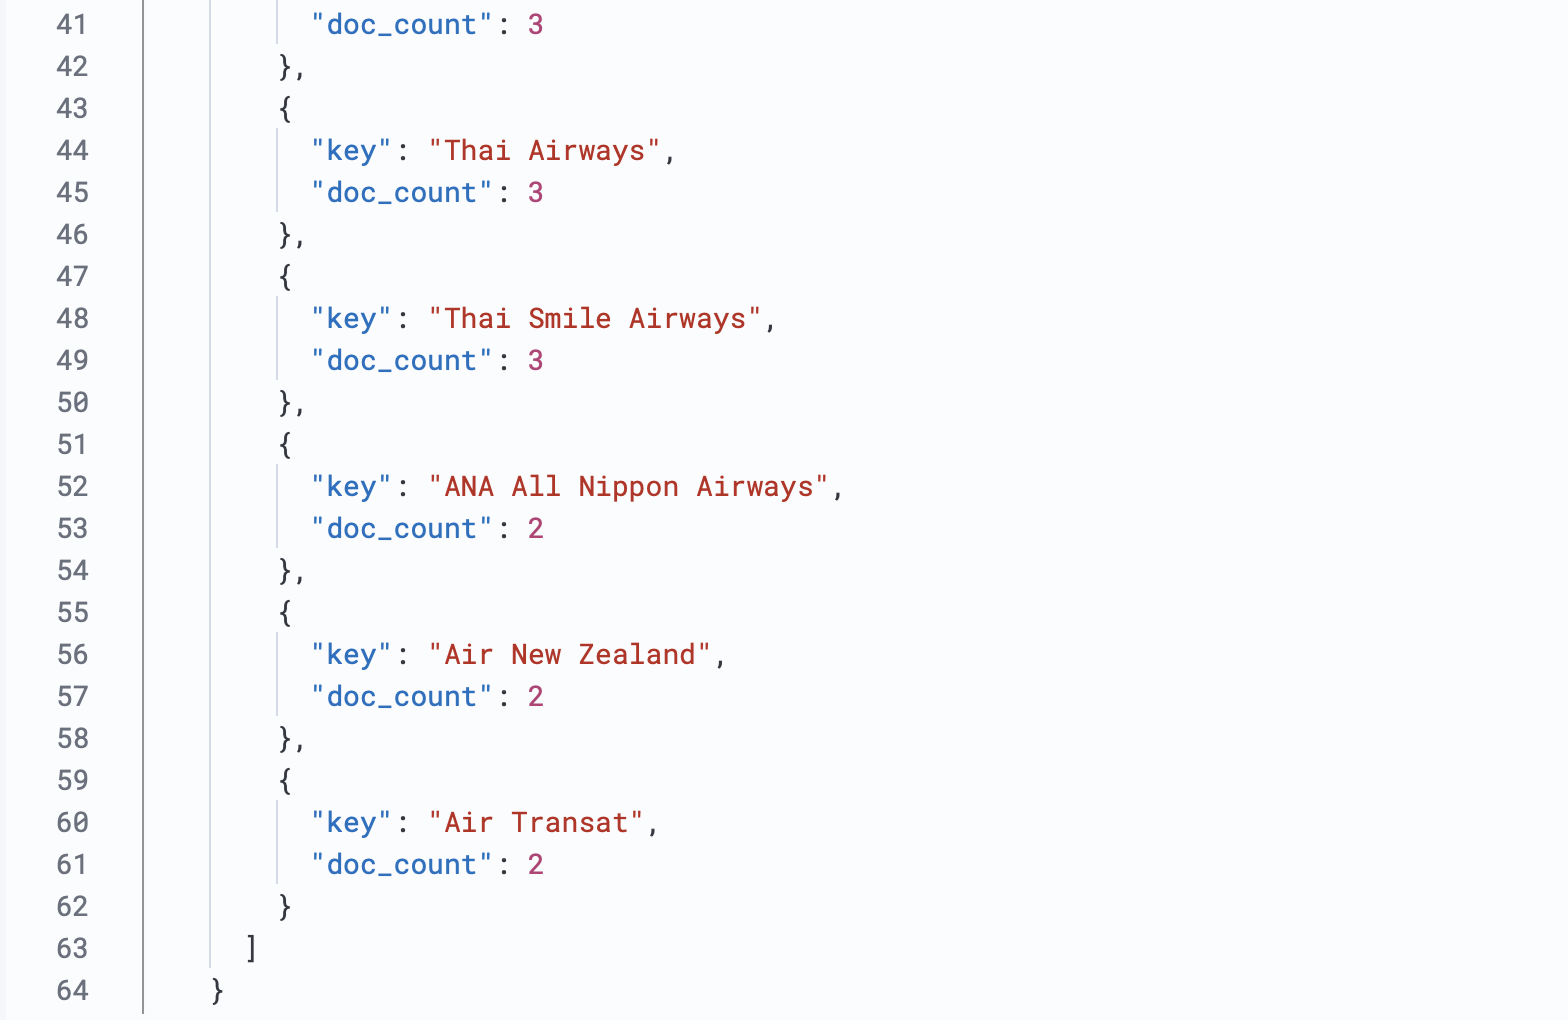
\includegraphics[scale=0.50]{Images/QueryResults/query3b.png}
    }
    \caption{Results from Query 3}

\end{figure}

\newpage

    \item Get the list of the airlines names and their respective number of reviews regarding baggage or luggage lost, for flights flying from, to or via Frankfurt

\begin{verbatim}
GET airlines/_search
{
  "size": 0,
  "query": {
    "bool": {
    "must": [
      {
        "match": {
          "Route": "Frankfurt"
        }
      },
      {
        "match": {
          "Review": "The luggages were lost"
        }
      },
      {
        "match": {
          "Review": "The baggages were lost"
        }
      }
    ]
    }
  },
  "aggs": {
    "lost_per_airlines": {
      "terms": {
        "field": "Airline Name"
      }
    }
  }
}
\end{verbatim}
\newpage
\begin{figure}[H]
    \centering
    \subfloat{
        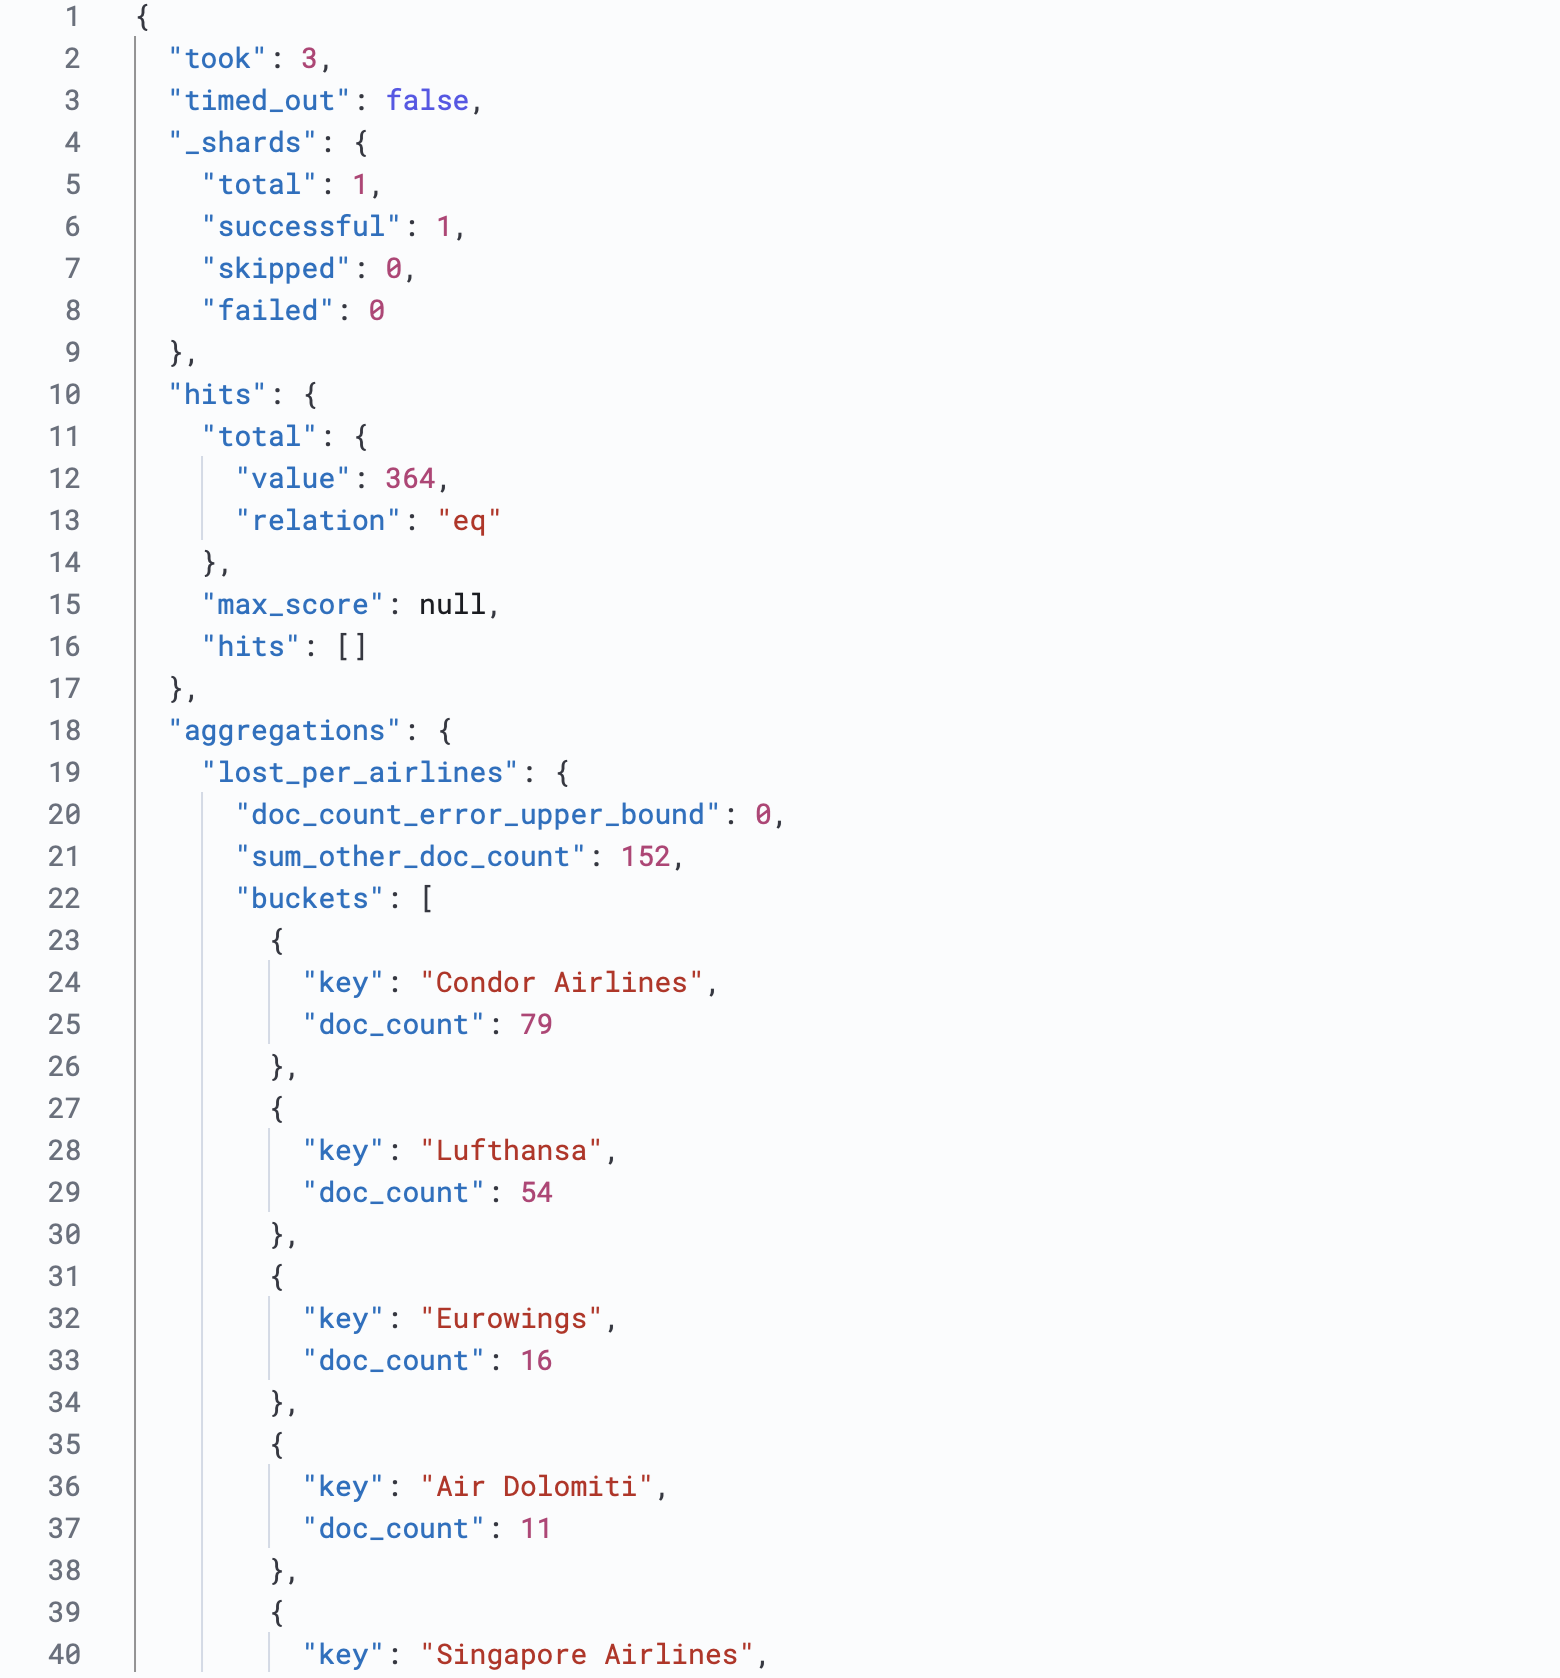
\includegraphics[scale=0.50]{Images/QueryResults/query4a.png}
    }\\
    \subfloat{
        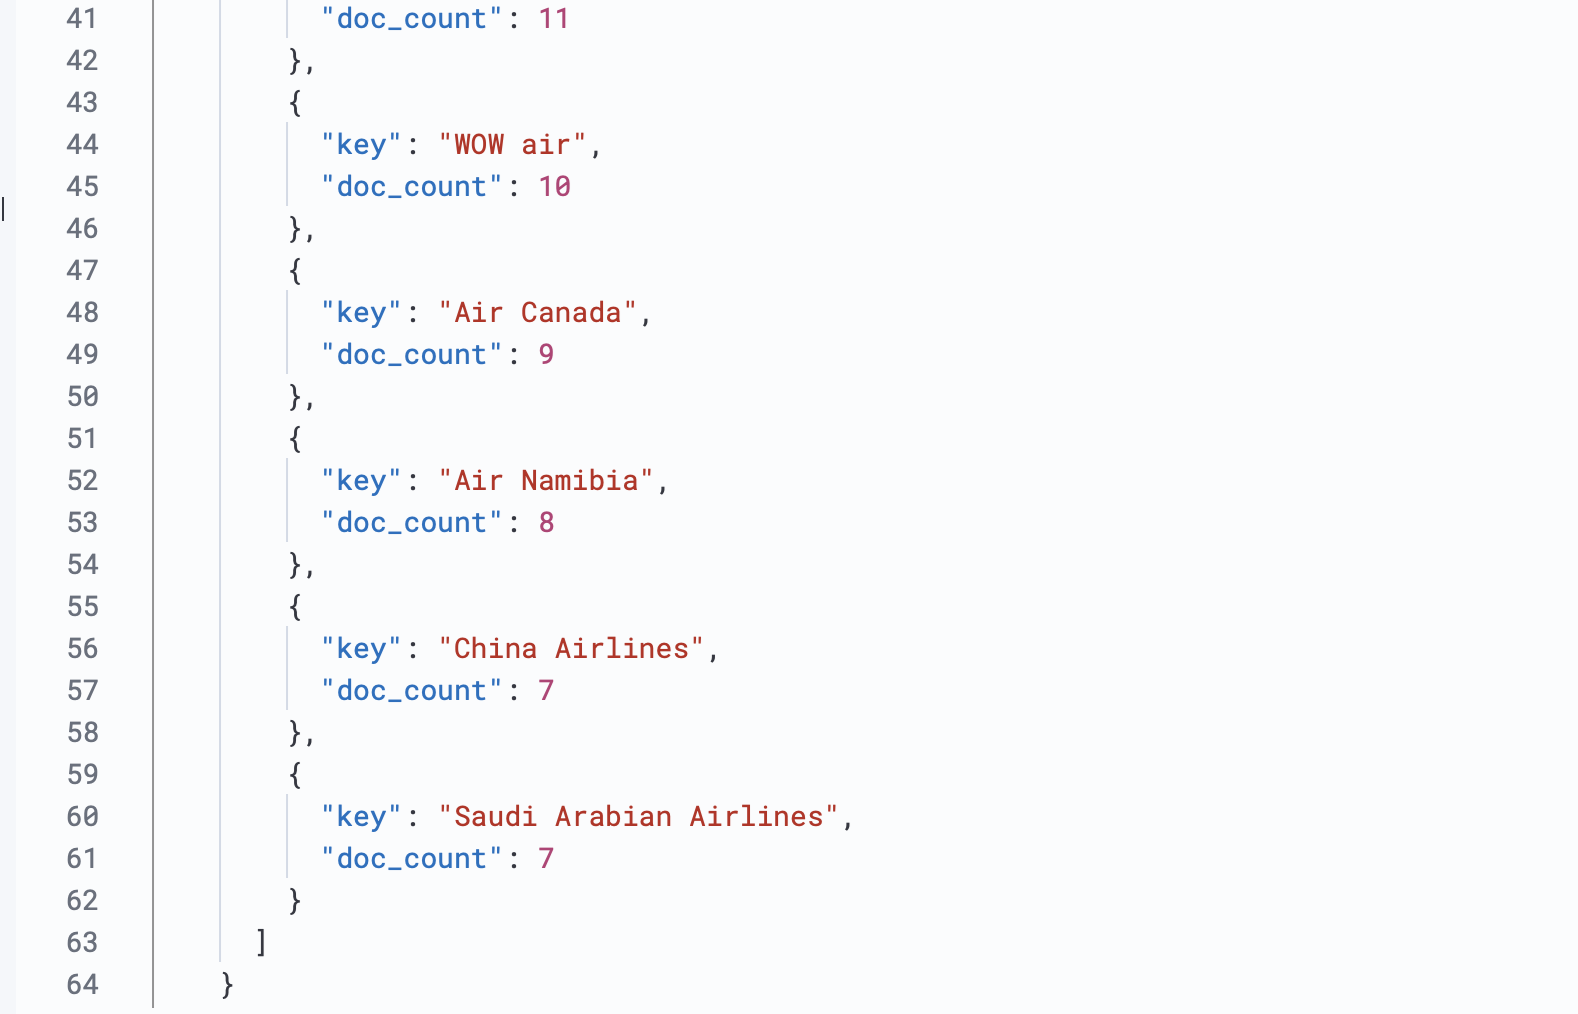
\includegraphics[scale=0.50]{Images/QueryResults/query4b.png}
    }
    \caption{Results from Query 4}

\end{figure}

\newpage

    \item Get the list of the reviews talking about a delay on a short flight, filtering out the reviews who recommend the airline, possibly telling it was a bad experience.

\begin{verbatim}
GET airlines/_search
{
  "query": {
    "bool": {
      "filter": {
        "term": {
        "Recommended": false
        }
      },
      "must": [
        {
          "match": {
            "Review": "Delay"
          }
        }, 
          {
            "match": {
              "Review": "Short Flight"
            }
        }
      ],
      "should": [
        {
          "match": {"Review": "Bad, horrible, terrible experience"}
        }
      ]
    }
  }
}
\end{verbatim}

\begin{figure}[H]
    \centering
    \subfloat{
        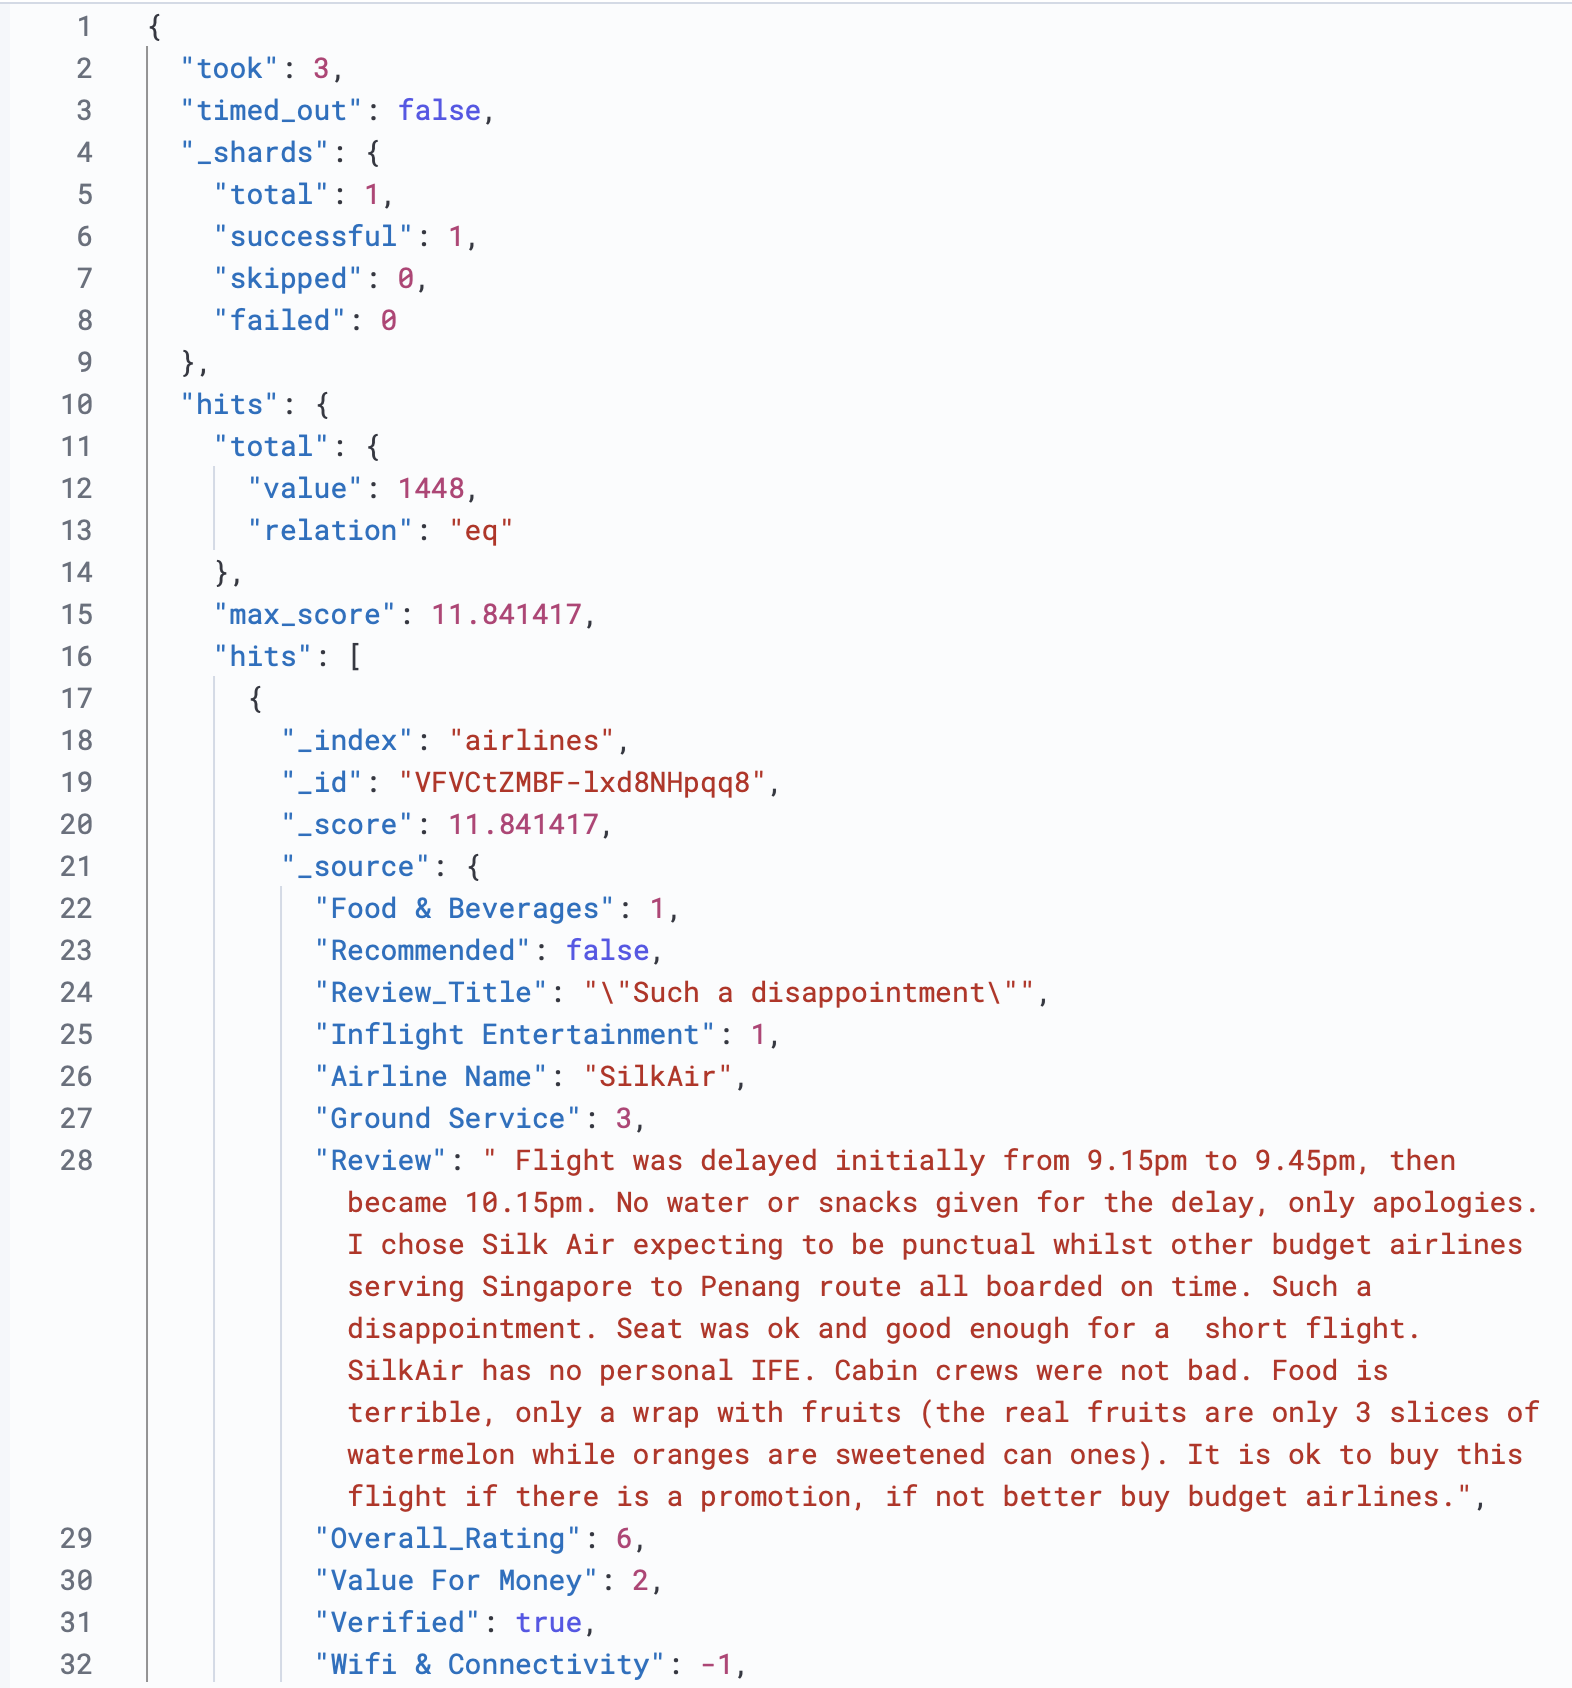
\includegraphics[scale=0.27]{Images/QueryResults/query5a.png}
    }\\
    
    \subfloat{
        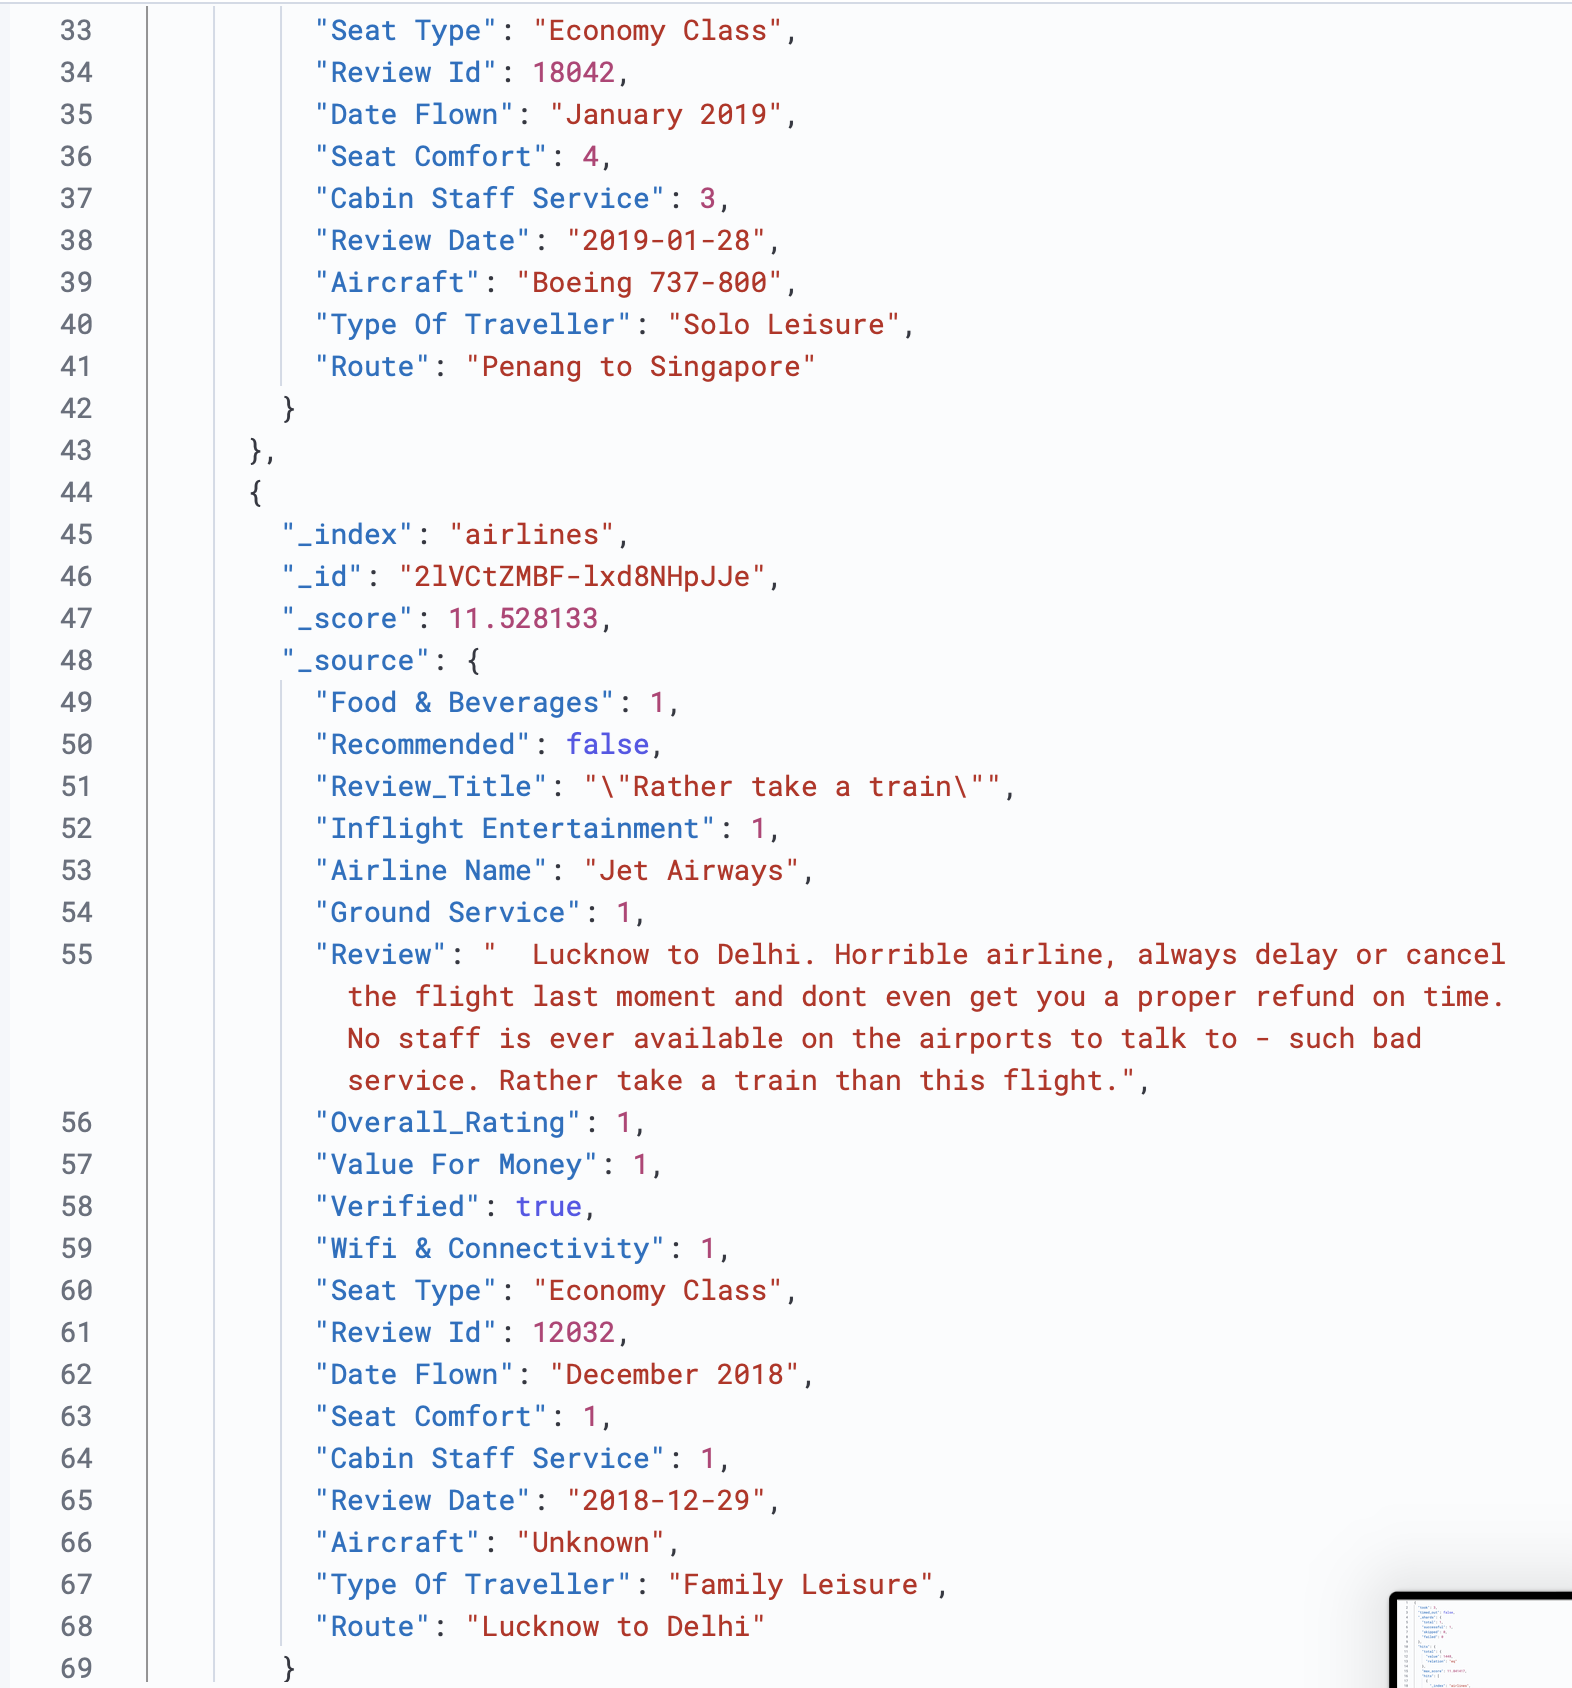
\includegraphics[scale=0.27]{Images/QueryResults/query5b.png}
    }\\
    \subfloat{
        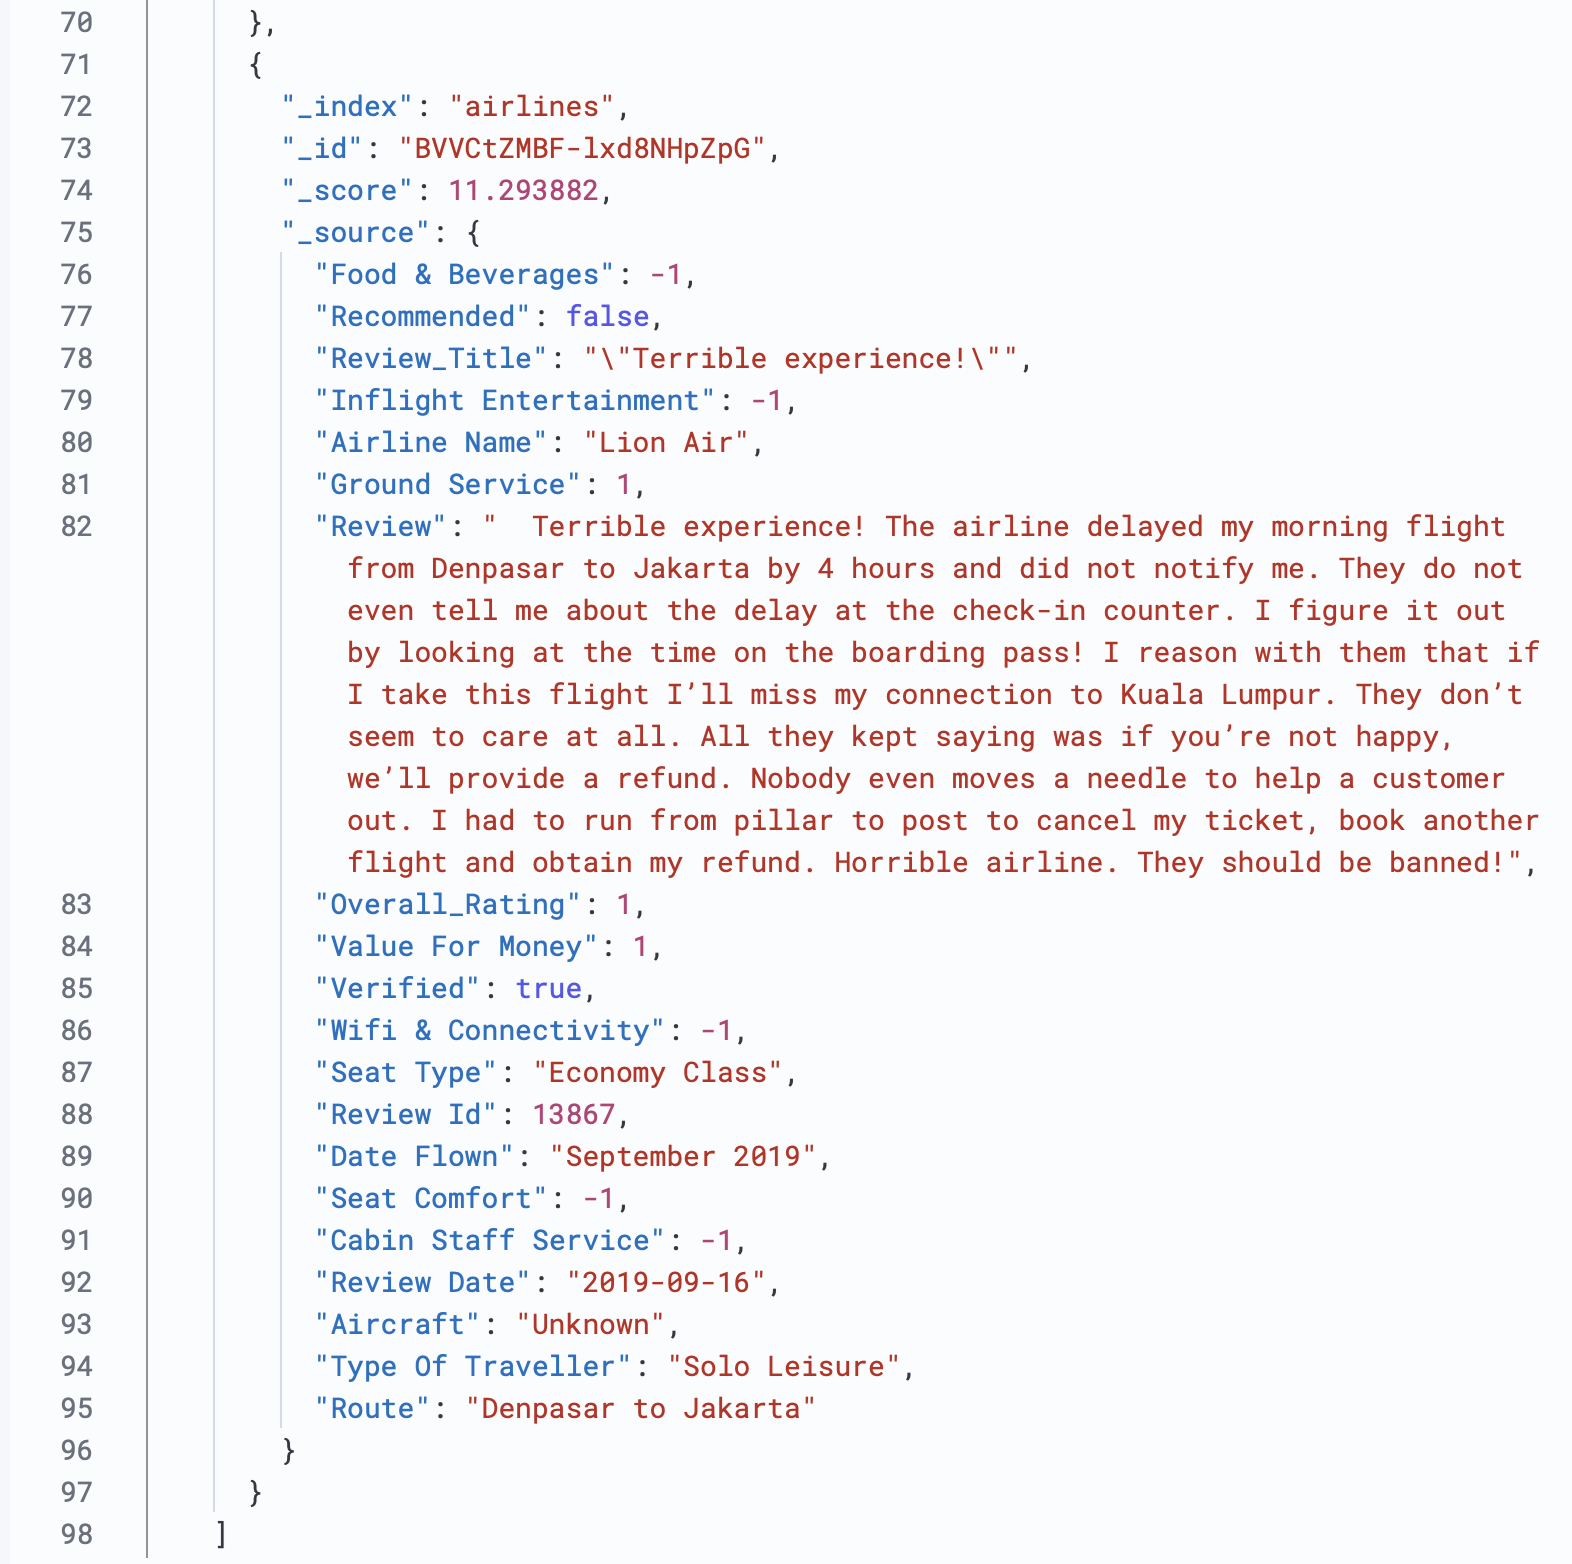
\includegraphics[scale=0.27]{Images/QueryResults/query5c.png}
    }
    \caption{Results from Query 5}

\end{figure}

\newpage

    \item Get the list of airlines lexicographically sorted together with the average of the seat comfort score (Notice That: you must not count in the average the reviews that have null values: -1 is considered a null value)
    \begin{verbatim}
GET airlines/_search
{
  "size": 0,
  "query": {
    "bool": {
      "filter": {
        "range": {
        "Seat Comfort": {
          "gte": 1
          }
        }
      }
    }
  }, 
  "aggs": {
    "avg_rating_by_traveller_type": {
      "terms": {
        "field": "Airline Name",
        "order": {
            "_key": "asc"
          }
      },
      "aggs": {
        "avg_overall_rating": {
          "avg": {
            "field": "Seat Comfort"
          }
        }
      }
    }
  }
}
\end{verbatim}
\begin{figure}[H]
    \centering
    \subfloat{
        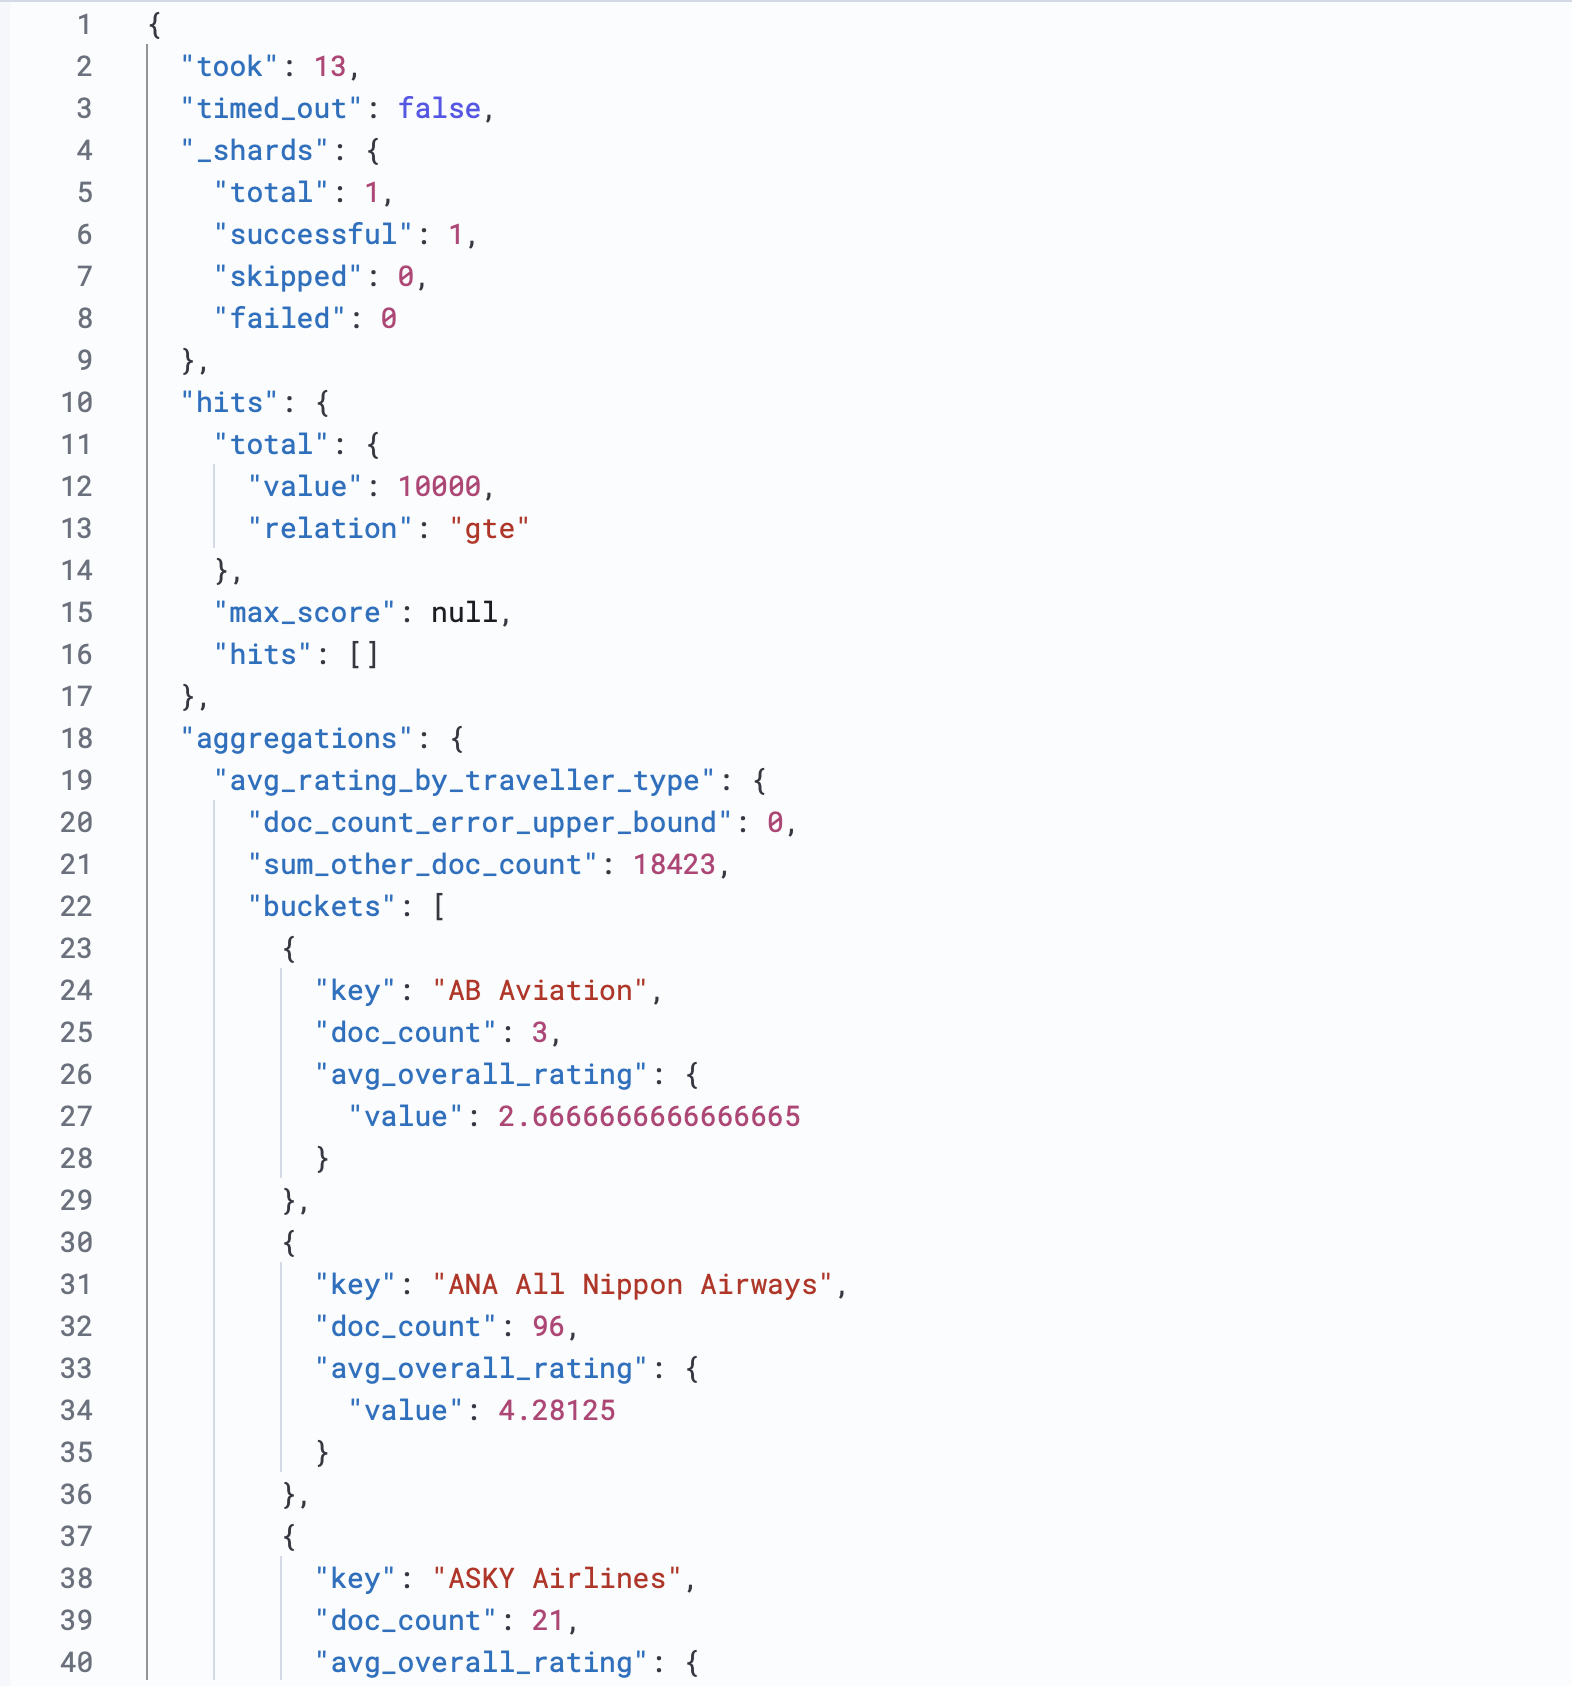
\includegraphics[scale=0.28]{Images/QueryResults/query6a.png}
    }
    \quad
    \subfloat{
        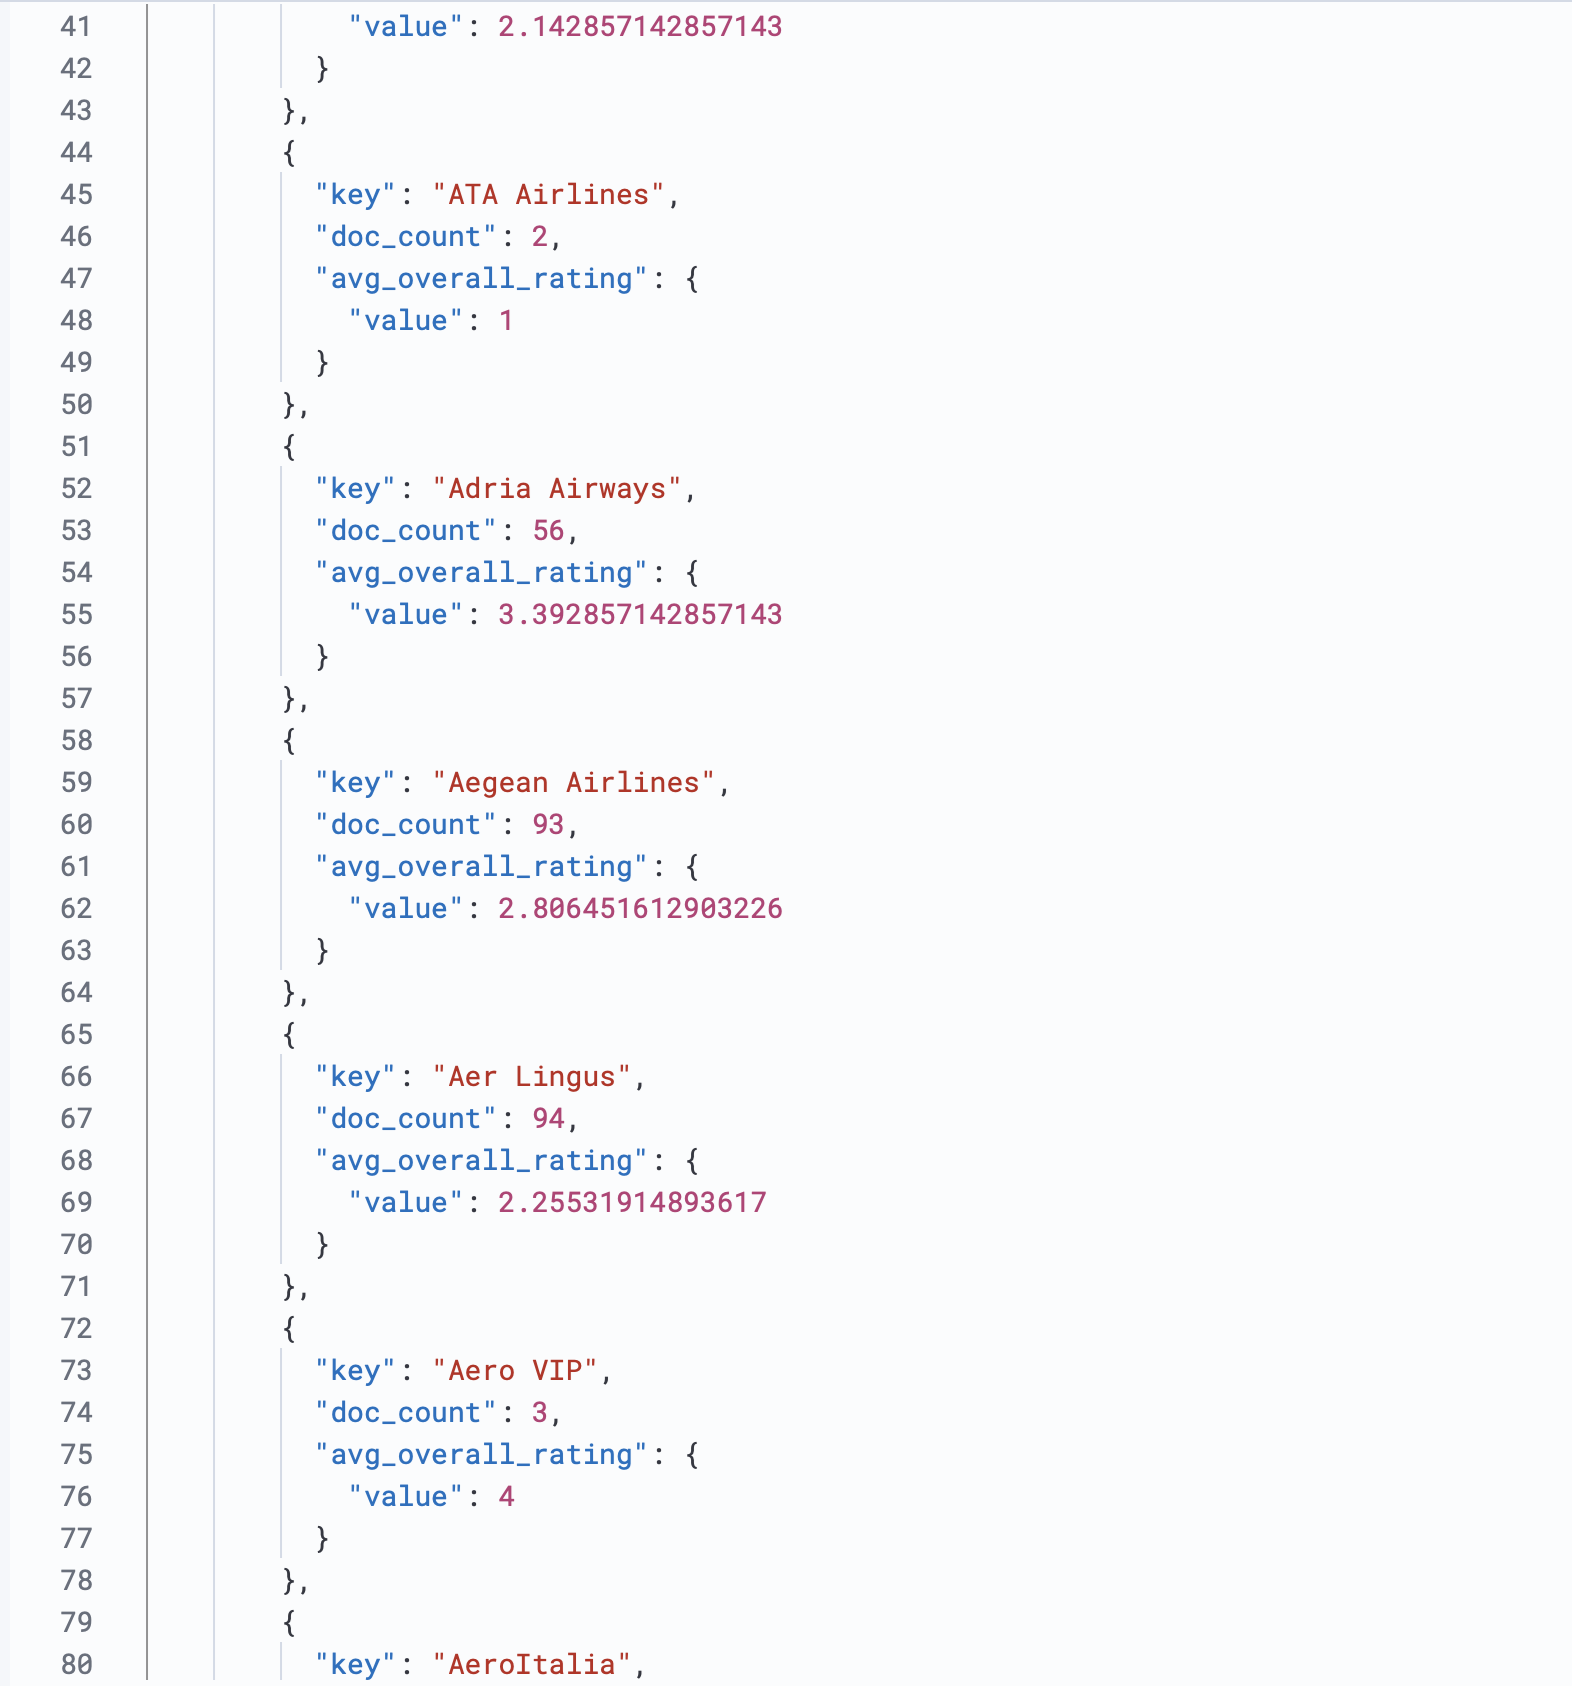
\includegraphics[scale=0.28]{Images/QueryResults/query6b.png}
    }
    \quad
    \subfloat{
        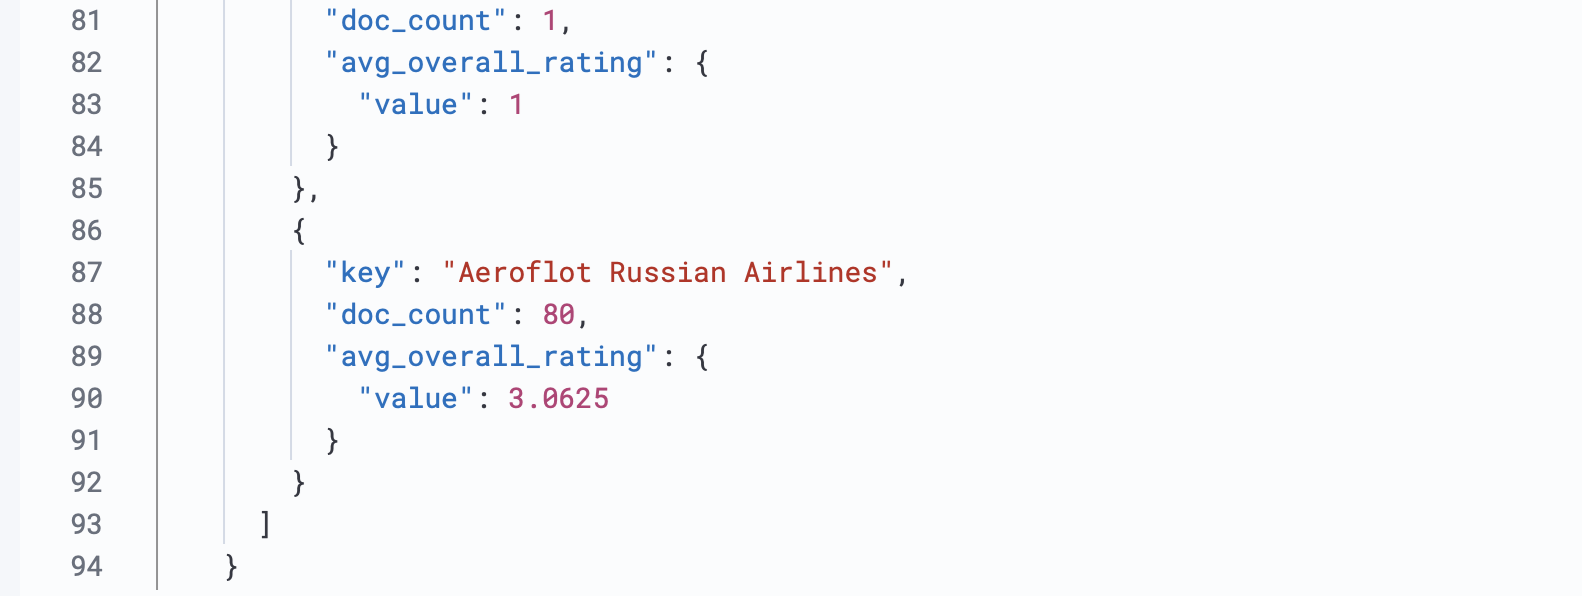
\includegraphics[scale=0.28]{Images/QueryResults/query6c.png}
    }
    \caption{Results from Query 5}

\end{figure}

\newpage

    \item Group the reviews by their seat type and find their average score, sorting the results by ascending average

    \begin{verbatim}
GET airlines/_search
{
  "size": 0,
  "aggs": {
    "avg_rating_by_traveller_type": {
      "terms": {
        "field": "Seat Type",
        "order": {
            "avg_overall_rating": "asc"
          }
      },
      "aggs": {
        "avg_overall_rating": {
          "avg": {
            "field": "Overall_Rating"
          }
        }
      }
    }
  }
}

    \end{verbatim}


\begin{figure}[H]
    \centering
    \subfloat{
        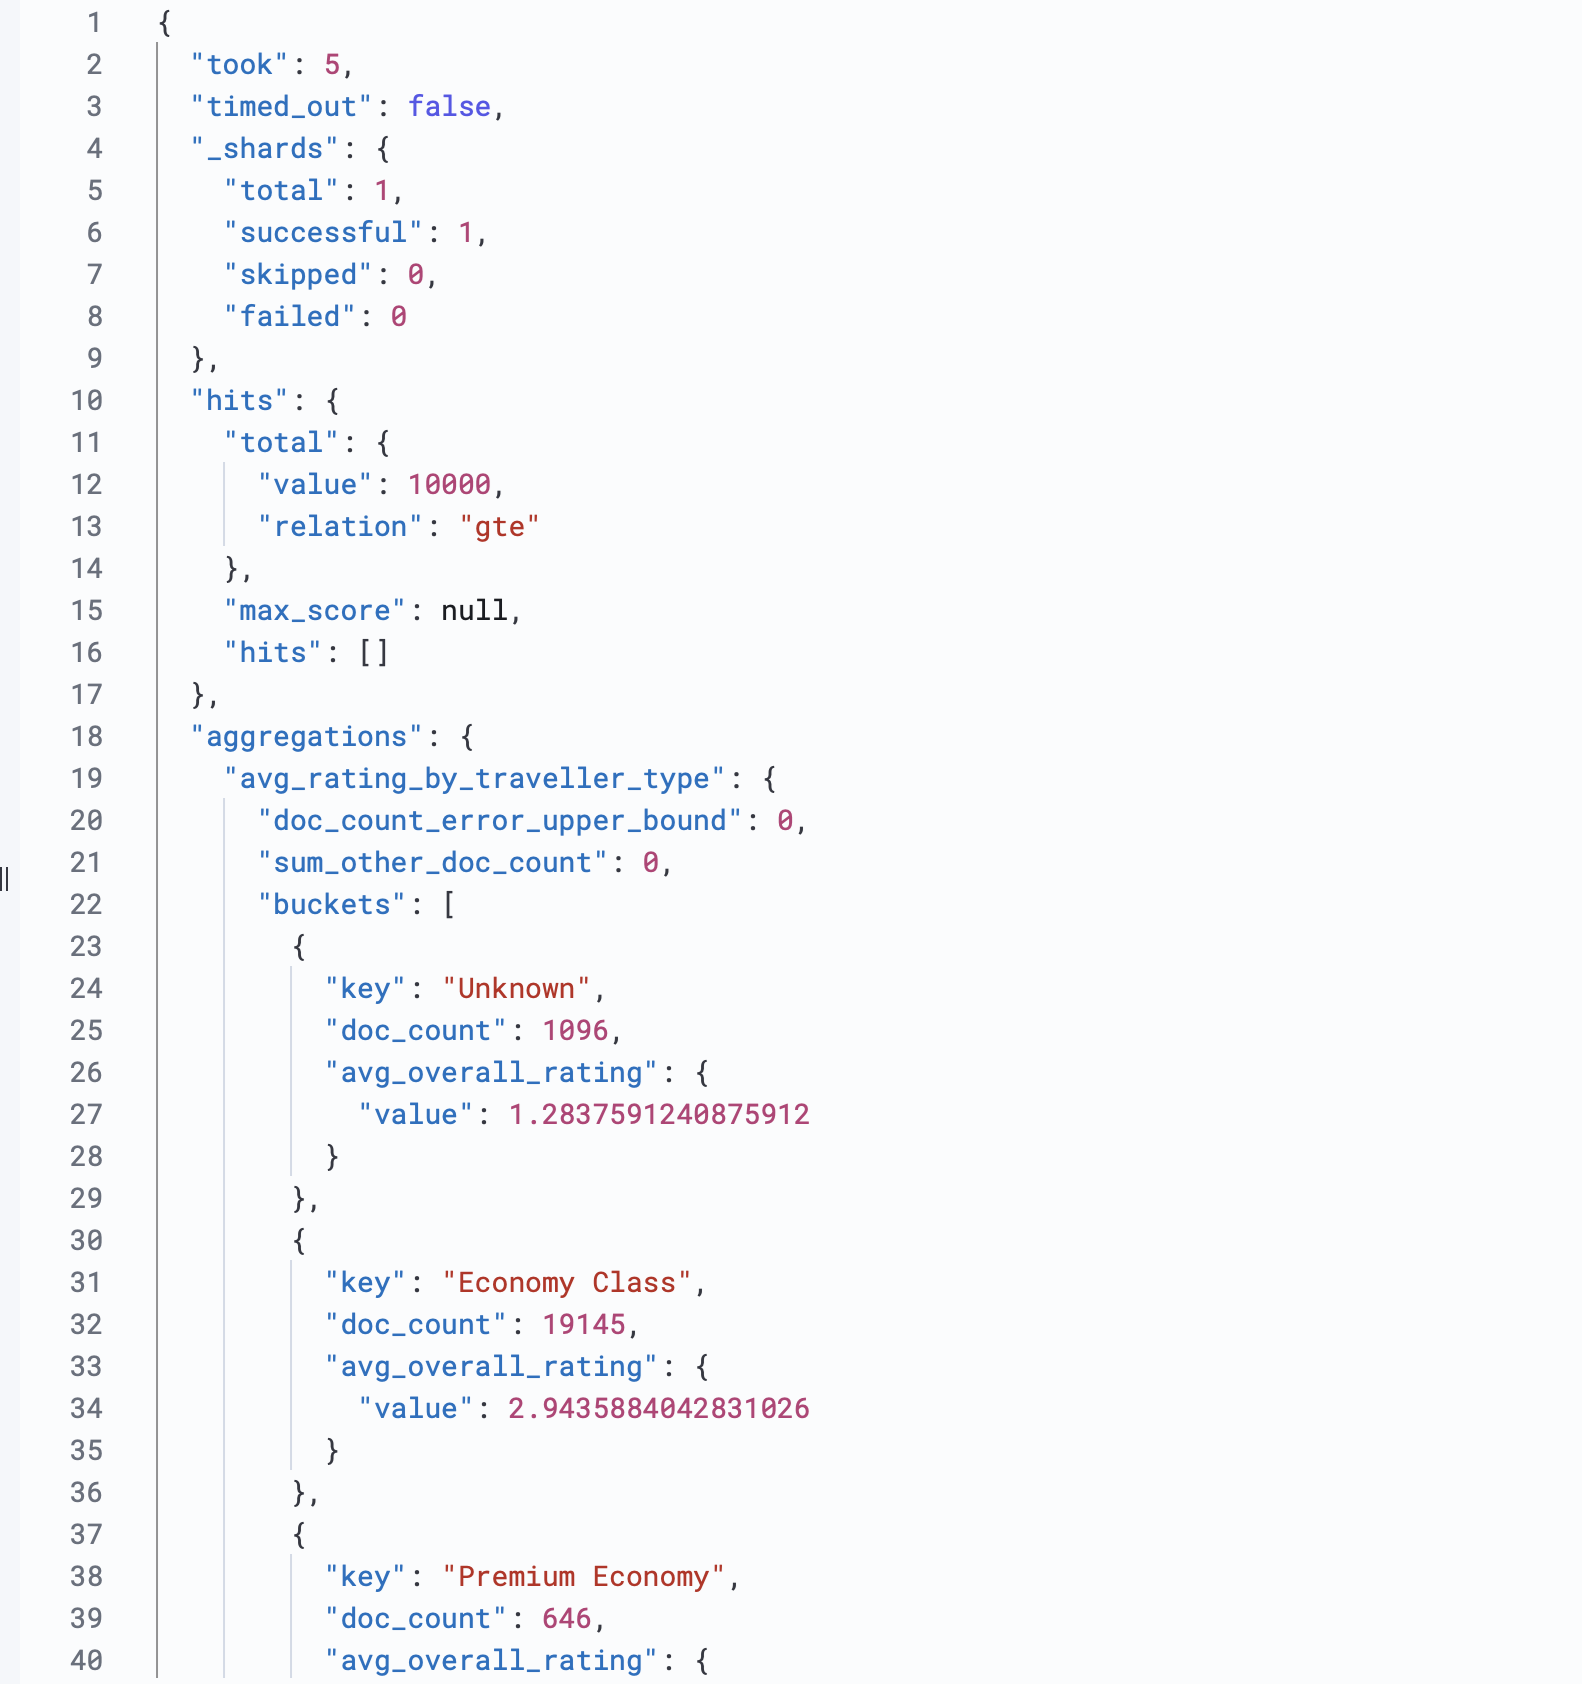
\includegraphics[scale=0.50]{Images/QueryResults/query7a.png}
    }
    \quad
    \subfloat{
        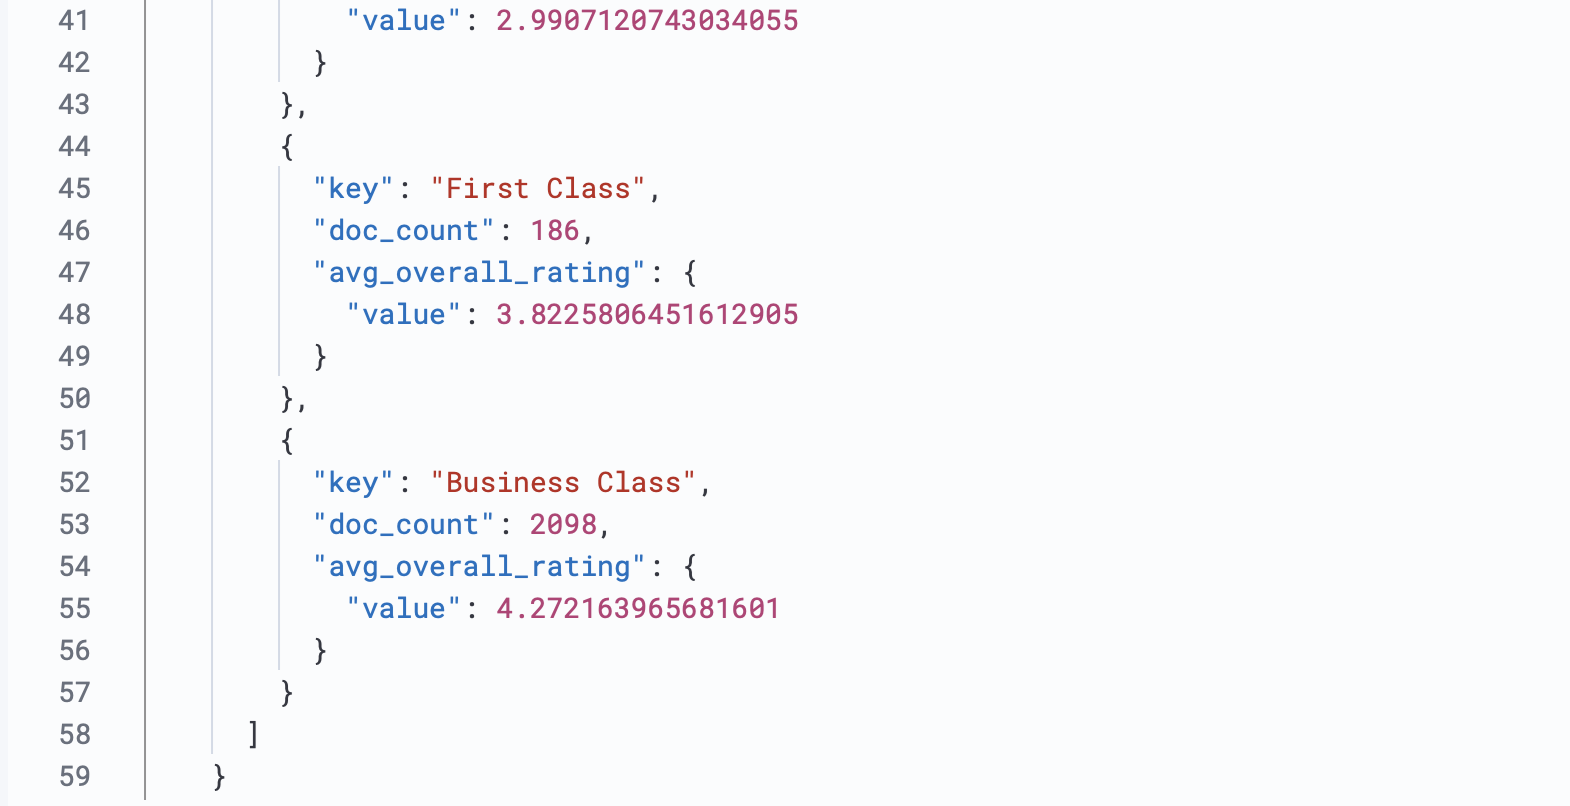
\includegraphics[scale=0.50]{Images/QueryResults/query7b.png}
    }
        \caption{Results from Query 7}

\end{figure}

    \item Count the number of reviews per month in the year 2022 and sort the months in ascendant order by number of reviews

    \begin{verbatim}
GET airlines/_search
{
  "size": 0,
  "query": {
    "bool": {
      "filter": {
        "wildcard": {
          "Date Flown": "*2022"
        }
      }
    }
  },
  "aggs": {
    "reviews_by_month": {
      "terms": {
        "field": "Date Flown",
        "order": {
          "_count": "asc"
        },
        "size": 12
      }
    }
  }
}
    \end{verbatim}

Query results:
\begin{figure}[H]
    \centering
    \subfloat{
        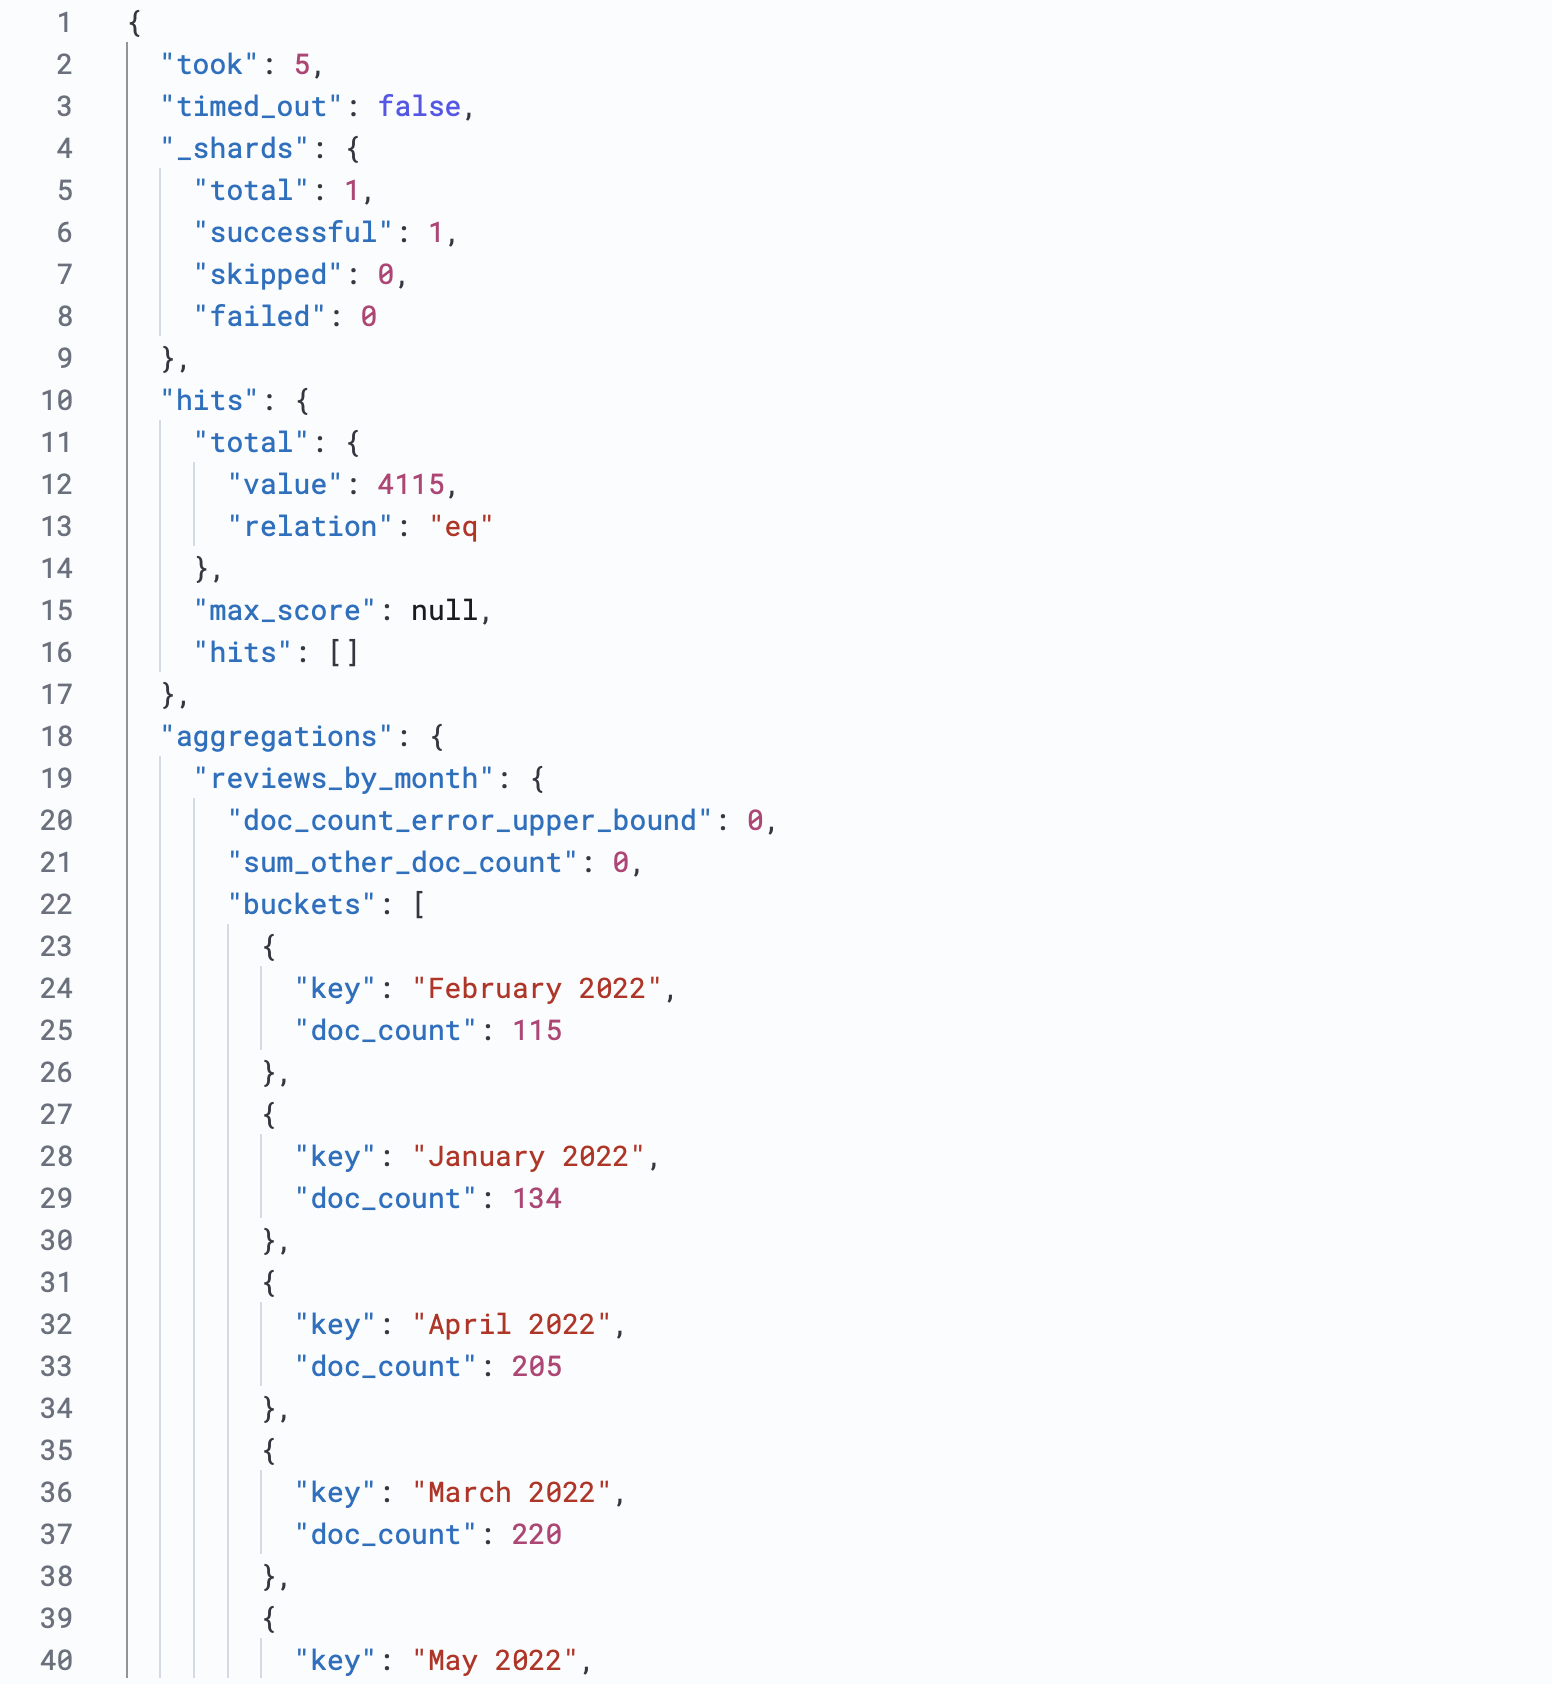
\includegraphics[scale=0.40]{Images/QueryResults/query8a.png}
    }
    \quad
    \subfloat{
        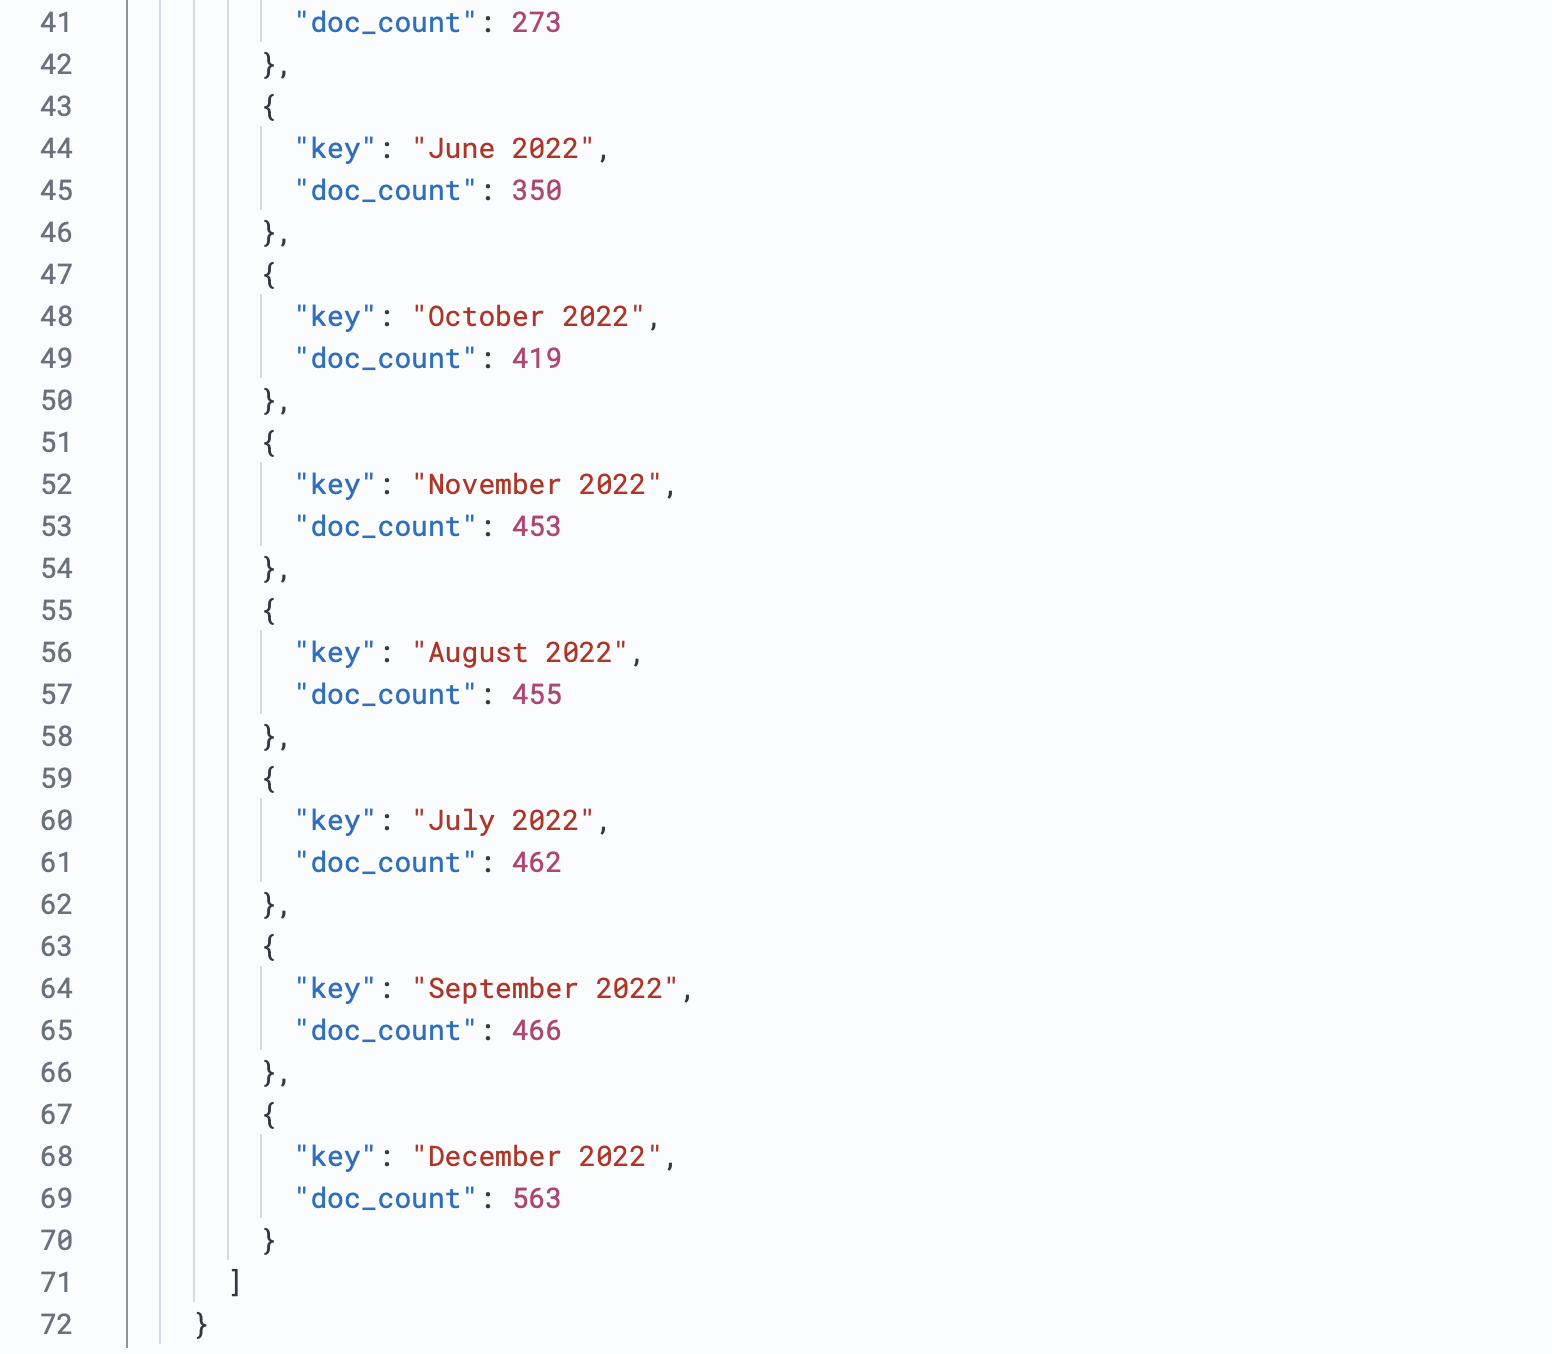
\includegraphics[scale=0.40]{Images/QueryResults/query8b.png}
    }
        \caption{Results from Query 5}

\end{figure}

\newpage

    \item Get the 10 worst airlines for average total rating calculated only on airlines that have at least 20 reviews and whose score is not null (-1 is considered a null value)

    \begin{verbatim}
GET /airlines/_search
{
  "query": {
    "bool": {
      "must_not": {
        "term": {
          "Overall_Rating": -1
        }
      }
    }
  },
  "aggs": {
    "group_by_airline": {
      "terms": {
        "field": "Airline Name",
        "size": 1000000, 
        "min_doc_count": 20
      },
      "aggs": {
        "avg_rating": {
          "avg": {
            "field": "Overall_Rating"
          }
        },
        "sort_by_avg_rating": {
          "bucket_sort": {
            "sort": [
              {
                "avg_rating": {
                  "order": "asc"  
                }
              }
            ],
            "size": 10 
          }
        }
      }
    }
  },
  "size": 0
}

    \end{verbatim}
\newpage
    \begin{figure}[H]
    \centering
    \subfloat{
        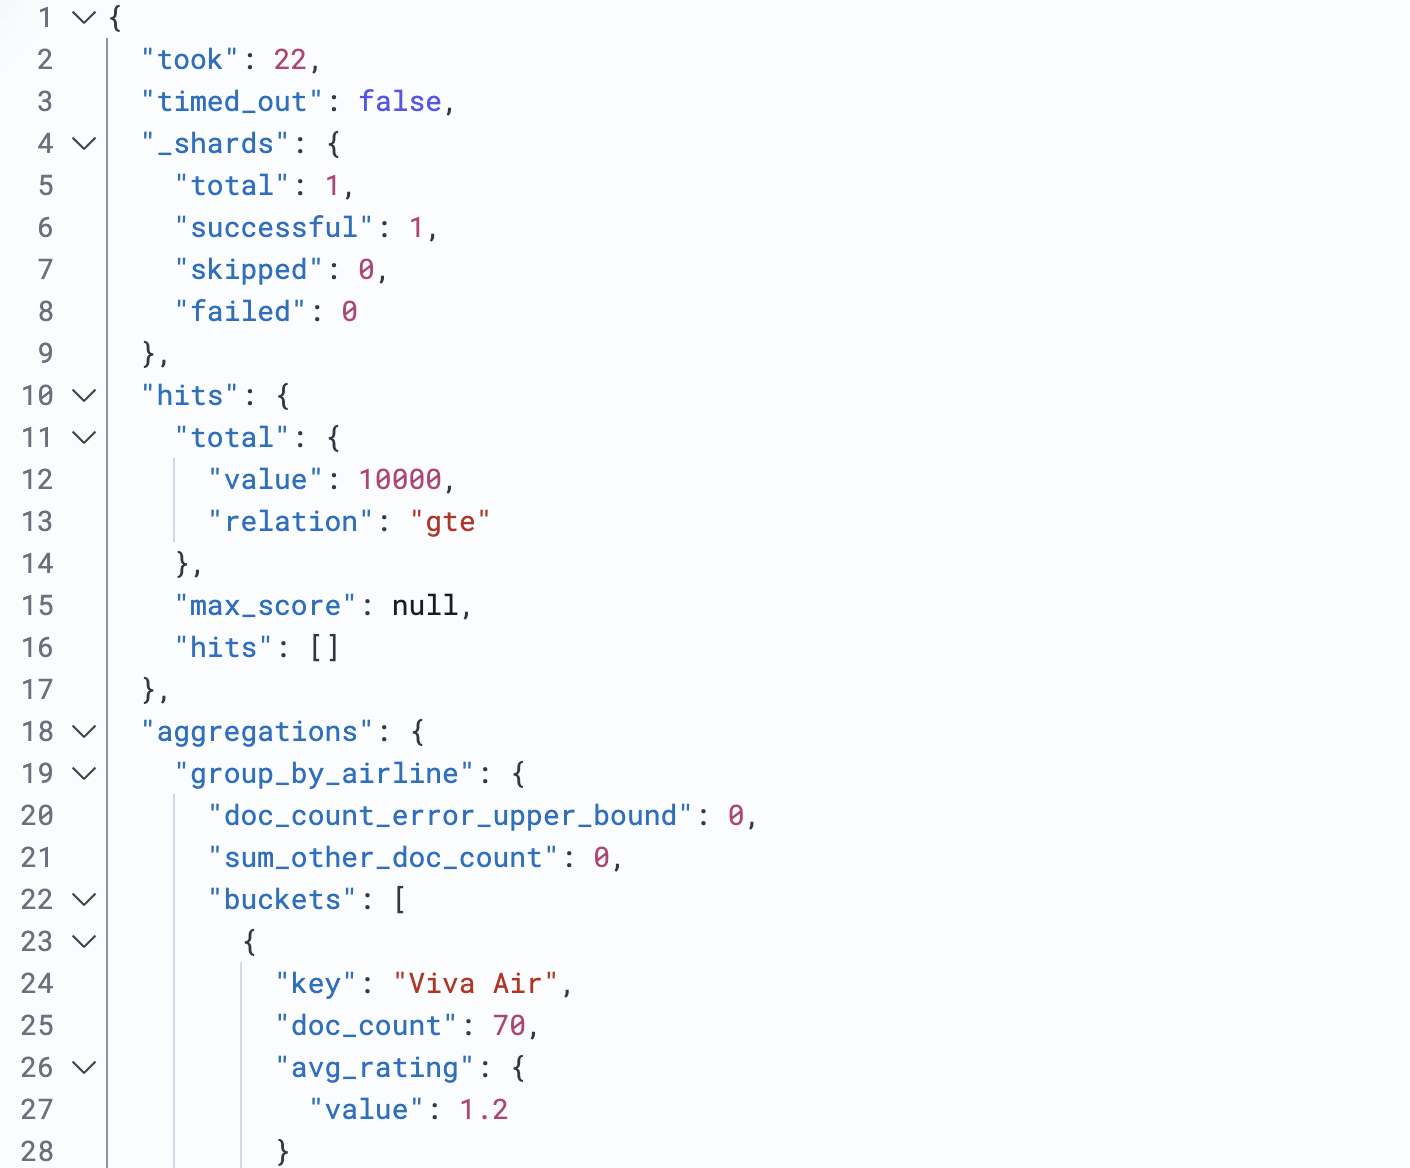
\includegraphics[scale=0.4]{Images/QueryResults/query9a.png}
    }
    \quad
    \subfloat{
        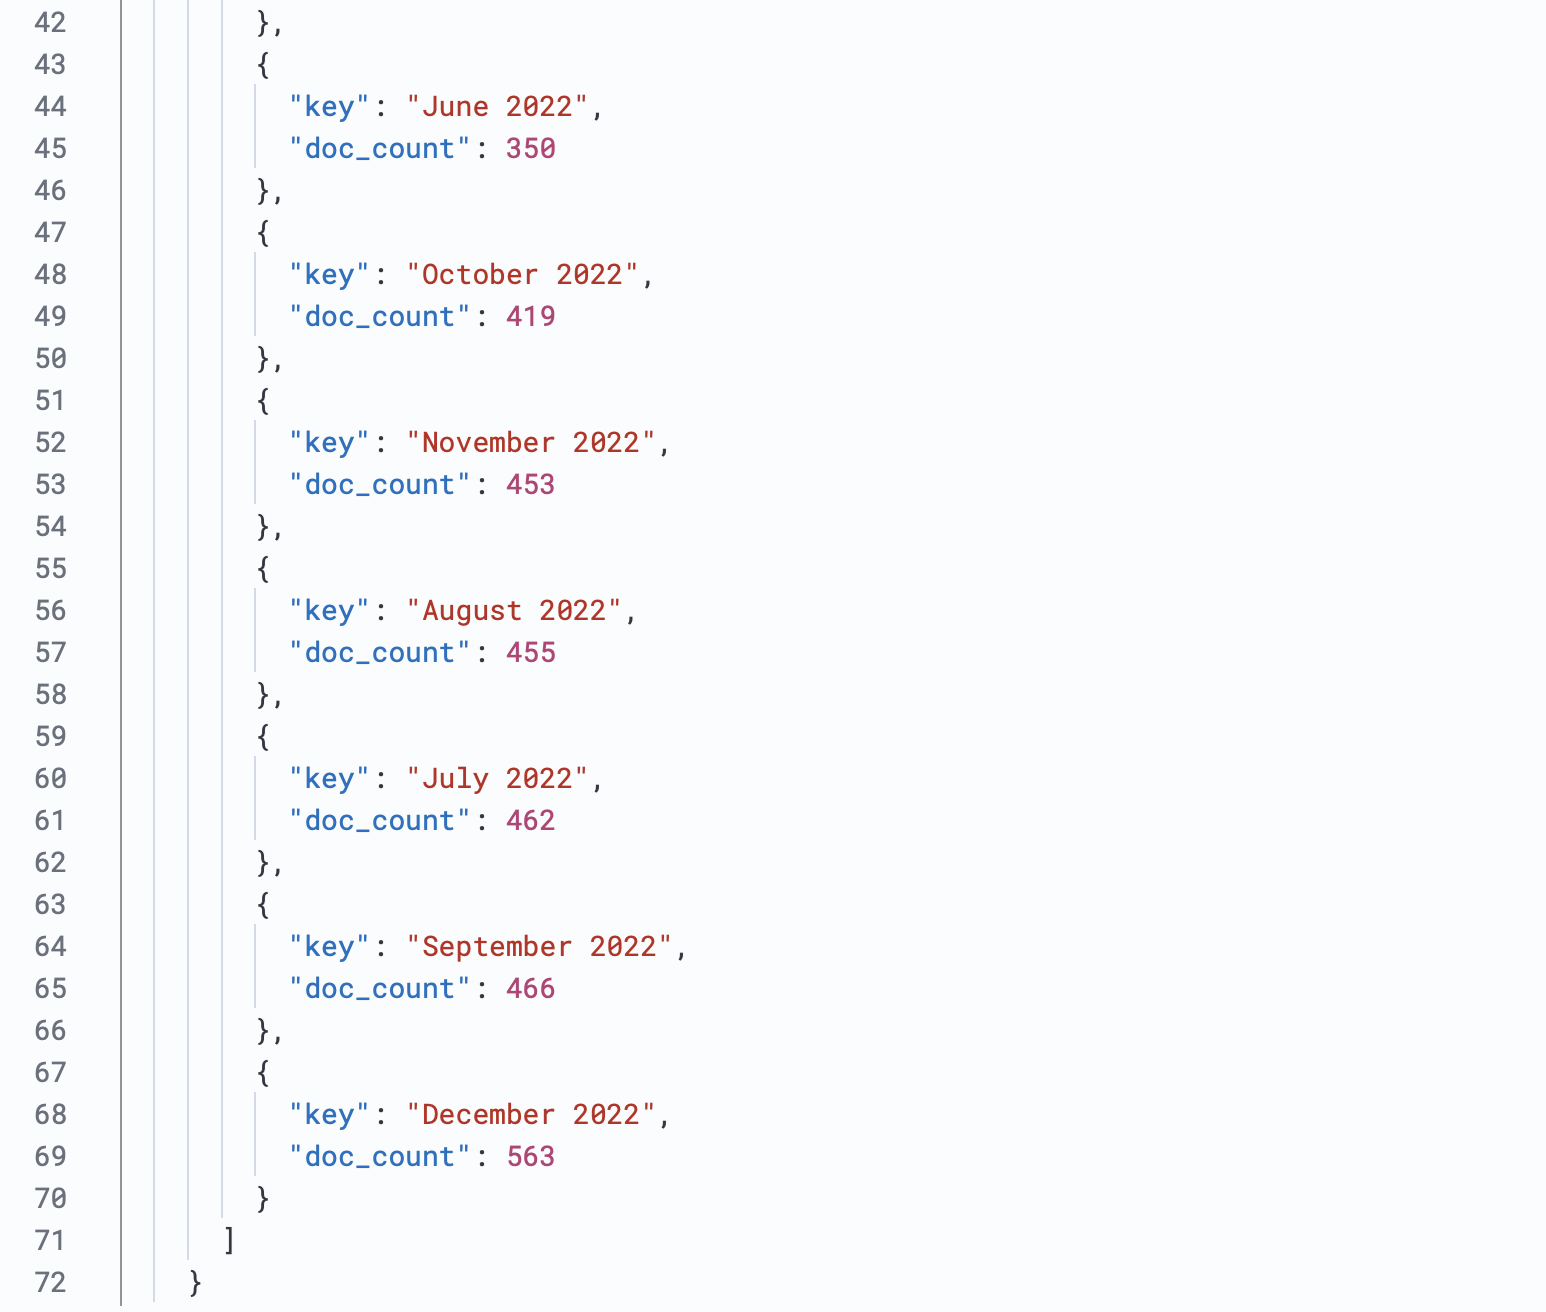
\includegraphics[scale=0.4]{Images/QueryResults/query9b.png}
    }
    \caption{Results from Query 9}

\end{figure}

\newpage
    
    \item Get the best x airlines by overall rating average that had at least 7 reviews, without considering the reviews having Value for money null (-1 is considered a null value)

    \begin{verbatim}
        
GET airlines/_search
{
  "size": 0,
  "query": {
    "bool": {
      "filter": {
        "range": {
          "Value For Money": {
            "gte": 0
          }
        }
      }
    }
  },
  "aggs": {
    "avg_rating_airline": {
      "terms": {
        "field": "Airline Name",
        "size": 10,
        "order": {
          "airlines_avg": "desc"
        },
        "min_doc_count": 7
      },
      "aggs": {
        "airlines_avg": {
          "avg": {
            "field": "Value For Money"
          }
        }
      }
    }
  }}
    \end{verbatim}
\end{enumerate}
% \label{sec:section_name}
% Chapters are typically subdivided into sections and subsections, and, optionally,
% subsubsections, paragraphs and subparagraphs.
% All can have a title, but only sections and subsections are numbered.
% A new section is created by the command
% \begin{verbatim}
% \section{Title of the section}
% \end{verbatim}
% The numbering can be turned off by using \verb|\section*{}|.
% \\
% A new subsection is created by the command
% \begin{verbatim}
% \subsection{Title of the subsection}
% \end{verbatim}
% and, similarly, the numbering can be turned off by adding an asterisk as follows 
% \begin{verbatim}
% \subsection*{}
% \end{verbatim}

% \section{Equations}
% \label{sec:eqs}
% This section gives some examples of writing mathematical equations in your thesis.

% Maxwell's equations read:
% \begin{subequations}
%     \label{eq:maxwell}
%     \begin{align}[left=\empheqlbrace]
%     \nabla\cdot \bm{D} & = \rho, \label{eq:maxwell1} \\
%     \nabla \times \bm{E} +  \frac{\partial \bm{B}}{\partial t} & = \bm{0}, \label{eq:maxwell2} \\
%     \nabla\cdot \bm{B} & = 0, \label{eq:maxwell3} \\
%     \nabla \times \bm{H} - \frac{\partial \bm{D}}{\partial t} &= \bm{J}. \label{eq:maxwell4}
%     \end{align}
% \end{subequations}

% Equation~\eqref{eq:maxwell} is automatically labeled by \texttt{cleveref},
% as well as Equation~\eqref{eq:maxwell1} and Equation~\eqref{eq:maxwell3}.
% Thanks to the \verb|cleveref| package, there is no need to use \verb|\eqref|.
% Remember that Equations have to be numbered only if they are referenced in the text.

% Equations~\eqref{eq:maxwell_multilabels1}, \eqref{eq:maxwell_multilabels2}, \eqref{eq:maxwell_multilabels3}, and \eqref{eq:maxwell_multilabels4} show again Maxwell's equations without brace:
% \begin{align}
%     \nabla\cdot \bm{D} & = \rho, \label{eq:maxwell_multilabels1} \\
%     \nabla \times \bm{E} +  \frac{\partial \bm{B}}{\partial t} &= \bm{0}, \label{eq:maxwell_multilabels2} \\
%     \nabla\cdot \bm{B} & = 0, \label{eq:maxwell_multilabels3} \\
%     \nabla \times \bm{H} - \frac{\partial \bm{D}}{\partial t} &= \bm{J} \label{eq:maxwell_multilabels4}.
% \end{align}

% Equation~\eqref{eq:maxwell_singlelabel} is the same as before,
% but with just one label:
% \begin{equation}
%     \label{eq:maxwell_singlelabel}
%     \left\{
%     \begin{aligned}
%     \nabla\cdot \bm{D} & = \rho, \\
%     \nabla \times \bm{E} +  \frac{\partial \bm{B}}{\partial t} &= \bm{0},\\
%     \nabla\cdot \bm{B} & = 0, \\
%     \nabla \times \bm{H} - \frac{\partial \bm{D}}{\partial t} &= \bm{J}.
%     \end{aligned}
%     \right.
% \end{equation}

% \section{Figures, Tables and Algorithms}
% Figures, Tables and Algorithms have to contain a Caption that describe their content, and have to be properly reffered in the text.

% \subsection{Figures}
% \label{subsec:figures}

% For including pictures in your text you can use \texttt{TikZ} for high-quality hand-made figures,
% or just include them as usual with the command
% \begin{verbatim}
% \includegraphics[options]{filename.xxx}
% \end{verbatim}
% Here xxx is the correct format, e.g. \verb|.png|, \verb|.jpg|, \verb|.eps|, \dots.

% \begin{figure}[H]
%     \centering
%     
\includegraphics[width=0.3\textwidth]{logo_polimi_scritta.eps}
%     \caption{Caption of the Figure to appear in the List of Figures.}
%     \label{fig:quadtree}
% \end{figure}

% Thanks to the \texttt{\textbackslash subfloat} command, a single figure, such as Figure~\ref{fig:quadtree},
% can contain multiple sub-figures with their own caption and label, e.g. \color{black} Figure~\ref{fig:polimi_logo1} and Figure~\ref{fig:polimi_logo2}. 

% \begin{figure}[H]
%     \centering
%     \subfloat[One PoliMi logo.\label{fig:polimi_logo1}]{
%         
\includegraphics[scale=0.5]{Images/logo_polimi_scritta.eps}
%     }
%     \quad
%     \subfloat[Another one PoliMi logo.\label{fig:polimi_logo2}]{
%         
\includegraphics[scale=0.5]{Images/logo_polimi_scritta2.eps}
%     }
%     \caption[Shorter caption]{This is a very long caption you don't want to appear in the List of Figures.}
%     \label{fig:quadtree2}
% \end{figure}


% \subsection{Tables}
% \label{subsec:tables}

% Within the environments \texttt{table} and  \texttt{tabular} you can create very fancy tables as the one shown in Table~\ref{table:example}.
% \begin{table}[H]
%     \caption*{\textbf{Title of Table (optional)}}
%     \centering 
%     \begin{tabular}{|p{3em} c c c |}
%     \hline
%     \rowcolor{bluepoli!40} % comment this line to remove the color
%      & \textbf{column 1} & \textbf{column 2} & \textbf{column 3} \T\B \\
%     \hline \hline
%     \textbf{row 1} & 1 & 2 & 3 \T\B \\
%     \textbf{row 2} & $\alpha$ & $\beta$ & $\gamma$ \T\B\\
%     \textbf{row 3} & alpha & beta & gamma \B\\
%     \hline
%     \end{tabular}
%     \\[10pt]
%     \caption{Caption of the Table to appear in the List of Tables.}
%     \label{table:example}
% \end{table}

% You can also consider to highlight selected columns or rows in order to make tables more readable.
% Moreover, with the use of \texttt{table*} and the option \texttt{bp} it is possible to align them at the bottom of the page. One example is presented in Table~\ref{table:exampleC}. 

% \begin{table}[H]
% \centering 
%     \begin{tabular}{|p{3em} | c | c | c | c | c | c|}
%     \hline
% %    \rowcolor{bluepoli!40}
%      & \textbf{column1} & \textbf{column2} & \textbf{column3} & \textbf{column4} & \textbf{column5} & \textbf{column6} \T\B \\
%     \hline \hline
%     \textbf{row1} & 1 & 2 & 3 & 4 & 5 & 6 \T\B\\
%     \textbf{row2} & a & b & c & d & e & f \T\B\\
%     \textbf{row3} & $\alpha$ & $\beta$ & $\gamma$ & $\delta$ & $\phi$ & $\omega$ \T\B\\
%     \textbf{row4} & alpha & beta & gamma & delta & phi & omega \B\\
%     \hline
%     \end{tabular}
%     \\[10pt]
%     \caption{Highlighting the columns}
%     \label{table:exampleC}
% \end{table}

% \begin{table}[H]
% \centering 
%     \begin{tabular}{|p{3em} c c c c c c|}
%     \hline
% %    \rowcolor{bluepoli!40}
%      & \textbf{column1} & \textbf{column2} & \textbf{column3} & \textbf{column4} & \textbf{column5} & \textbf{column6} \T\B \\
%     \hline \hline
%     \textbf{row1} & 1 & 2 & 3 & 4 & 5 & 6 \T\B\\
%     \hline
%     \textbf{row2} & a & b & c & d & e & f \T\B\\
%     \hline
%     \textbf{row3} & $\alpha$ & $\beta$ & $\gamma$ & $\delta$ & $\phi$ & $\omega$ \T\B\\
%     \hline
%     \textbf{row4} & alpha & beta & gamma & delta & phi & omega \B\\
%     \hline
%     \end{tabular}
%     \\[10pt]
%     \caption{Highlighting the rows}
%     \label{table:exampleR}
% \end{table}

% \subsection{Algorithms}
% \label{subsec:algorithms}

% Pseudo-algorithms can be written in \LaTeX{} with the \texttt{algorithm} and \texttt{algorithmic} packages.
% An example is shown in Algorithm~\ref{alg:var}.
% \begin{algorithm}[H]
%     \label{alg:example}
%     \caption{Name of the Algorithm}
%     \label{alg:var}
%     \label{protocol1}
%     \begin{algorithmic}[1]
%     \STATE Initial instructions
%     \FOR{$for-condition$}
%     \STATE{Some instructions}
%     \IF{$if-condition$}
%     \STATE{Some other instructions}
%     \ENDIF
%     \ENDFOR
%     \WHILE{$while-condition$}
%     \STATE{Some further instructions}
%     \ENDWHILE
%     \STATE Final instructions
%     \end{algorithmic}
% \end{algorithm} 

% \vspace{5mm}

% \section{Theorems, propositions and lists}

% \subsection{Theorems}
% Theorems have to be formatted as:
% \begin{theorem}
% \label{a_theorem}
% Write here your theorem. 
% \end{theorem}
% \textit{Proof.} If useful you can report here the proof.

% \subsection{Propositions}
% Propositions have to be formatted as:
% \begin{proposition}
% Write here your proposition.
% \end{proposition}

% \subsection{Lists}
% How to  insert itemized lists:
% \begin{itemize}
%     \item first item;
%     \item second item.
% \end{itemize}
% How to insert numbered lists:
% \begin{enumerate}
%     \item first item;
%     \item second item.
% \end{enumerate}

%-------------------------------------------------------------------------
%	APPENDICES
%-------------------------------------------------------------------------

% \cleardoublepage
% \addtocontents{toc}{\vspace{2em}} % Add a gap in the Contents, for aesthetics
% \appendix
% \chapter{Appendix A}
% If you need to include an appendix to support the research in your thesis, you can place it at the end of the manuscript.
% An appendix contains supplementary material (figures, tables, data, codes, mathematical proofs, surveys, \dots)
% which supplement the main results contained in the previous chapters.


% LIST OF FIGURES
\listoffigures

% % LIST OF TABLES
% \listoftables

\cleardoublepage

\end{document}
